%DIF 1-2d1
%DIF LATEXDIFF DIFFERENCE FILE
%DIF DEL ../rom_sciAdvances.tex    Sun Nov 18 07:30:14 2018
%DIF ADD rom_sciAdvances_rev.tex   Thu Dec 20 11:40:11 2018
%DIF < % Use only LaTeX2e, calling the article.cls class and 12-point type.
%DIF < 
%DIF -------
\documentclass[12pt]{article}

%DIF 5-10d3
%DIF < % Users of the {thebibliography} environment or BibTeX should use the
%DIF < % scicite.sty package, downloadable from *Science* at
%DIF < % http://www.sciencemag.org/authors/preparing-manuscripts-using-latex 
%DIF < % This package should properly format in-text
%DIF < % reference calls and reference-list numbers.
%DIF < 
%DIF -------
\usepackage{scicite}
\let\citep=\cite

% \usepackage{times}

%DIF 16-20d8
%DIF < % The preamble here sets up a lot of new/revised commands and
%DIF < % environments.  It's annoying, but please do *not* try to strip these
%DIF < % out into a separate .sty file (which could lead to the loss of some
%DIF < % information when we convert the file to other formats).  Instead, keep
%DIF < % them in the preamble of your main LaTeX source file.
%DIF -------

\usepackage{graphicx}
\usepackage{authblk}
\usepackage{lineno}
\usepackage{paralist}
\usepackage{amsmath}

%DIF 28-33d15
%DIF < %% for citing stuff in the supp
%DIF < % \usepackage{xr}
%DIF < % \externaldocument{rom_sciAdvances_supp}
%DIF < 
%DIF < % The following parameters seem to provide a reasonable page setup.
%DIF < 
%DIF -------
\topmargin 0.0cm
\oddsidemargin 0.2cm
\textwidth 16cm 
\textheight 21cm
\footskip 1.0cm


%DIF 41-42c22
%DIF < %The next command sets up an environment for the abstract to your paper.
%DIF < 
%DIF -------
% environment for the abstract %DIF > 
%DIF -------
\newenvironment{sciabstract} 
{\bfseries}
{}

% to include rmd output
\usepackage[final]{pdfpages}



%DIF 48a28-33
\title{Non-equilibrium evolution of volatility in origination and %DIF > 
  extinction explains fat-tailed fluctuations in Phanerozoic %DIF > 
  biodiversity \\ %DIF > 
  \vspace{1em} \large {\it One sentence summary:} Phanerozoic marine %DIF > 
  invertebrate richness fluctuates in a non-equilibrium process due to %DIF > 
  pulsed adaptive evolution.} %DIF > 
%DIF -------

%DIF 49-53d35
%DIF < % Include your paper's title here
%DIF < 
%DIF < \title{Non-equilibrium rate heterogeneity explains fat-tailed
%DIF <   fluctuations in Phanerozoic biodiversity}
%DIF < 
%DIF -------
\author[1, {*}]{Andrew J. Rominger}
\author[1, 2, 3]{Miguel A. Fuentes}
\author[1, 4, 5, 6, 7]{Pablo A. Marquet}

\affil[1]{\normalsize{Santa Fe Institute, 1399 Hyde Park Road, Santa Fe, New
Mexico 87501, US}}
%
\affil[2]{\normalsize{Instituto de Investigaciones Filos\'oficas, SADAF, CONICET,
Bulnes 642, 1428 Buenos Aires, Argentin}}
%
\affil[3]{\normalsize{Facultad de Ingenier\'ia y Tecnolog\'ia, Universidad San
Sebasti\'an, Lota 2465, Santiago 7510157, Chile}}
%
\affil[4]{\normalsize{Departamento de Ecolog\'ia, Facultad de Ciencias
Biol\'ogicas, Pontificia Universidad de Chile, Alameda 340, Santiago,
Chile}}
%
%DIF 71-72c52-53
%DIF < \affil[5]{\normalsize{Instituto de Ecolog\'ia y Biodiversidad, Casilla 653,
%DIF < Santiago, Chile}}
%DIF -------
\affil[5]{\normalsize{Instituto de Ecolog\'ia y Biodiversidad (IEB), %DIF > 
    Casilla 653, Santiago, Chile}} %DIF > 
%DIF -------
%
%DIF 74-76c55-57
%DIF < \affil[6]{\normalsize{Laboratorio Internacional de Cambio Global (LINCGlobal),
%DIF < Pontificia Universidad Católica de Chile, Alameda 340, Santiago,
%DIF < Chile}}
%DIF -------
\affil[6]{\normalsize{Laboratorio Internacional de Cambio Global %DIF > 
    (LINCGlobal), and Centro de Cambio Global UC, Pontificia %DIF > 
    Universidad Catolica de Chile, Santiago, Chile.}} %DIF > 
%DIF -------
%
%DIF 78-79c59-60
%DIF < \affil[7]{\normalsize{Centro Cambio Global UC, Av.~Vicu\~na Mackenna 4860, Campus
%DIF < San Vicu\~na, Santiago, Chile}}
%DIF -------
\affil[7]{\normalsize{Centro Cambio Global UC, Av.~Vicu\~na Mackenna %DIF > 
    4860, Campus San Vicu\~na, Santiago, Chile}} %DIF > 
%DIF -------
%
%DIF 81c62-66
%DIF < \affil[{*}]{\normalsize{To whom correspondence should be addressed; E-mail: rominger@santafe.edu}}
%DIF -------
\affil[8]{\normalsize{Centro de Ciencias de la Complejidad (C3), %DIF > 
    Universidad Nacional Aut\'onoma de M\'exico.}} %DIF > 
% %DIF > 
\affil[{*}]{\normalsize{To whom correspondence should be addressed, %DIF > 
    e-mail: rominger@santafe.edu}} %DIF > 
%DIF -------

\date{}



%DIF < %%%%%%%%%%%%%%%%% END OF PREAMBLE %%%%%%%%%%%%%%%%
%DIF -------
%%%% END OF PREAMBLE %%%% %DIF > 
%DIF PREAMBLE EXTENSION ADDED BY LATEXDIFF
%DIF UNDERLINE PREAMBLE %DIF PREAMBLE
\RequirePackage[normalem]{ulem} %DIF PREAMBLE
\RequirePackage{color}\definecolor{RED}{rgb}{1,0,0}\definecolor{BLUE}{rgb}{0,0,1} %DIF PREAMBLE
\providecommand{\DIFadd}[1]{{\color{blue}{#1}}} %DIF PREAMBLE
\providecommand{\DIFdel}[1]{{\protect\color{red}\sout{}}}                      %DIF PREAMBLE
%DIF SAFE PREAMBLE %DIF PREAMBLE
\providecommand{\DIFaddbegin}{} %DIF PREAMBLE
\providecommand{\DIFaddend}{} %DIF PREAMBLE
\providecommand{\DIFdelbegin}{} %DIF PREAMBLE
\providecommand{\DIFdelend}{} %DIF PREAMBLE
%DIF FLOATSAFE PREAMBLE %DIF PREAMBLE
\providecommand{\DIFaddFL}[1]{\DIFadd{#1}} %DIF PREAMBLE
\providecommand{\DIFdelFL}[1]{\DIFdel{#1}} %DIF PREAMBLE
\providecommand{\DIFaddbeginFL}{} %DIF PREAMBLE
\providecommand{\DIFaddendFL}{} %DIF PREAMBLE
\providecommand{\DIFdelbeginFL}{} %DIF PREAMBLE
\providecommand{\DIFdelendFL}{} %DIF PREAMBLE
\newcommand{\DIFscaledelfig}{0.5}
%DIF HIGHLIGHTGRAPHICS PREAMBLE %DIF PREAMBLE
\RequirePackage{settobox} %DIF PREAMBLE
\RequirePackage{letltxmacro} %DIF PREAMBLE
\newsavebox{\DIFdelgraphicsbox} %DIF PREAMBLE
\newlength{\DIFdelgraphicswidth} %DIF PREAMBLE
\newlength{\DIFdelgraphicsheight} %DIF PREAMBLE
% store original definition of \includegraphics %DIF PREAMBLE
\LetLtxMacro{\DIFOincludegraphics}{\includegraphics} %DIF PREAMBLE
\newcommand{\DIFaddincludegraphics}[2][]{{\color{blue}\fbox{\DIFOincludegraphics[#1]{#2}}}} %DIF PREAMBLE
\newcommand{\DIFdelincludegraphics}[2][]{% %DIF PREAMBLE
\sbox{\DIFdelgraphicsbox}{\DIFOincludegraphics[#1]{#2}}% %DIF PREAMBLE
\settoboxwidth{\DIFdelgraphicswidth}{\DIFdelgraphicsbox} %DIF PREAMBLE
\settoboxtotalheight{\DIFdelgraphicsheight}{\DIFdelgraphicsbox} %DIF PREAMBLE
\scalebox{\DIFscaledelfig}{% %DIF PREAMBLE
\parbox[b]{\DIFdelgraphicswidth}{\usebox{\DIFdelgraphicsbox}\\[-\baselineskip] \rule{\DIFdelgraphicswidth}{0em}}\llap{\resizebox{\DIFdelgraphicswidth}{\DIFdelgraphicsheight}{% %DIF PREAMBLE
\setlength{\unitlength}{\DIFdelgraphicswidth}% %DIF PREAMBLE
\begin{picture}(1,1)% %DIF PREAMBLE
\thicklines\linethickness{2pt} %DIF PREAMBLE
{\color[rgb]{1,0,0}\put(0,0){\framebox(1,1){}}}% %DIF PREAMBLE
{\color[rgb]{1,0,0}\put(0,0){\line( 1,1){1}}}% %DIF PREAMBLE
{\color[rgb]{1,0,0}\put(0,1){\line(1,-1){1}}}% %DIF PREAMBLE
\end{picture}% %DIF PREAMBLE
}\hspace*{3pt}}} %DIF PREAMBLE
} %DIF PREAMBLE
\LetLtxMacro{\DIFOaddbegin}{\DIFaddbegin} %DIF PREAMBLE
\LetLtxMacro{\DIFOaddend}{\DIFaddend} %DIF PREAMBLE
\LetLtxMacro{\DIFOdelbegin}{\DIFdelbegin} %DIF PREAMBLE
\LetLtxMacro{\DIFOdelend}{\DIFdelend} %DIF PREAMBLE
\DeclareRobustCommand{\DIFaddbegin}{\DIFOaddbegin \let\includegraphics\DIFaddincludegraphics} %DIF PREAMBLE
\DeclareRobustCommand{\DIFaddend}{\DIFOaddend \let\includegraphics\DIFOincludegraphics} %DIF PREAMBLE
\DeclareRobustCommand{\DIFdelbegin}{\DIFOdelbegin \let\includegraphics\DIFdelincludegraphics} %DIF PREAMBLE
\DeclareRobustCommand{\DIFdelend}{\DIFOaddend \let\includegraphics\DIFOincludegraphics} %DIF PREAMBLE
\LetLtxMacro{\DIFOaddbeginFL}{\DIFaddbeginFL} %DIF PREAMBLE
\LetLtxMacro{\DIFOaddendFL}{\DIFaddendFL} %DIF PREAMBLE
\LetLtxMacro{\DIFOdelbeginFL}{\DIFdelbeginFL} %DIF PREAMBLE
\LetLtxMacro{\DIFOdelendFL}{\DIFdelendFL} %DIF PREAMBLE
\DeclareRobustCommand{\DIFaddbeginFL}{\DIFOaddbeginFL \let\includegraphics\DIFaddincludegraphics} %DIF PREAMBLE
\DeclareRobustCommand{\DIFaddendFL}{\DIFOaddendFL \let\includegraphics\DIFOincludegraphics} %DIF PREAMBLE
\DeclareRobustCommand{\DIFdelbeginFL}{\DIFOdelbeginFL \let\includegraphics\DIFdelincludegraphics} %DIF PREAMBLE
\DeclareRobustCommand{\DIFdelendFL}{\DIFOaddendFL \let\includegraphics\DIFOincludegraphics} %DIF PREAMBLE
%DIF END PREAMBLE EXTENSION ADDED BY LATEXDIFF

\begin{document} 

%DIF <  Double-space the manuscript.
\DIFdelbegin %DIFDELCMD < 

%DIFDELCMD < \baselineskip24pt
%DIFDELCMD < 

%DIFDELCMD < %%%
%DIF <  Make the title.
%DIFDELCMD < 

%DIFDELCMD < %%%
\DIFdelend \maketitle 
\clearpage
\linenumbers

\begin{sciabstract}
  Fluctuations in biodiversity, both large and small, are pervasive
  through the fossil record, yet we do not understand the processes
  generating them.
% 
  Here we \DIFdelbegin \DIFdel{use a novel extension of }\DIFdelend \DIFaddbegin \DIFadd{extend }\DIFaddend theory from non-equilibrium statistical physics to
  \DIFdelbegin \DIFdel{show that three universal properties of
macroevolution---
%DIF < 
}%DIFDELCMD < \begin{inparaenum}[\itshape i\upshape)]
%DIFDELCMD < \item %%%
\DIFdel{heterogeneity of diversification rates between taxa, likely driven by 
}%DIFDELCMD < \item %%%
\DIFdel{niche conservatism and 
}%DIFDELCMD < \item %%%
\DIFdel{punctuated adaptive radiation---
}%DIFDELCMD < \end{inparaenum}
%DIFDELCMD < %%%
%DIF < 
\DIFdel{are sufficient to explain }\DIFdelend \DIFaddbegin \DIFadd{describe }\DIFaddend the previously unaccounted for fat-tailed form of
  fluctuations in \DIFdelbegin \DIFdel{diversity }\DIFdelend \DIFaddbegin \DIFadd{marine invertebrate richness }\DIFaddend through the
  Phanerozoic.
%
  Using this theory, known as superstatistics, we \DIFdelbegin \DIFdel{identify taxonomic
orders as largely autonomous evolutionary units, each likely
experiencing its own unique and conserved region of
  an adaptive
landscape. }\DIFdelend \DIFaddbegin \DIFadd{show that the simple
  fact of heterogeneous rates of origination and extinction between
  clades and conserved rates within clades is sufficient to account
  for this fat-tailed form. We identify orders and the families they
  subsume as the taxonomic level at which clades experience
  inter-clade heterogeneity and within clade homogeneity of
  rates. Following superstatistics we would thus posit that orders and
  families are subsystems in local statistical equilibrium while the
  entire system is not in equilibrium.
%DIF > 
  }\DIFaddend The separation of timescales between background origination and
  extinction \DIFaddbegin \DIFadd{within clades }\DIFaddend compared to the origin of major ecological
  and evolutionary innovations \DIFdelbegin \DIFdel{between orders allow within-order
}\DIFdelend \DIFaddbegin \DIFadd{leading to new orders and families
  allows within-clade }\DIFaddend dynamics to reach equilibrium, while
  \DIFdelbegin \DIFdel{between-order }\DIFdelend \DIFaddbegin \DIFadd{between-clade }\DIFaddend diversification is non-equilibrial\DIFdelbegin \DIFdel{, driven by major evolutionary innovations}\DIFdelend .
%
  \DIFaddbegin \DIFadd{This between clade non-equilibrium accounts for the fat-tailed
  nature of the system as a whole.
%DIF > 
  The distribution of shifts in diversification dynamics across orders
  and families is consistent with niche conservatism and pulsed
  exploration of adaptive landscapes by higher taxa.
%DIF > 
  }\DIFaddend Compared to other approaches that have used simple birth-death
  processes, \DIFaddbegin \DIFadd{simple }\DIFaddend equilibrial dynamics, or non-linear theories from
  complexity science, \DIFdelbegin \DIFdel{super-statistics }\DIFdelend \DIFaddbegin \DIFadd{superstatistics }\DIFaddend is superior in its ability to
  account for both small and extreme fluctuations in \DIFdelbegin \DIFdel{fossil diversity}\DIFdelend \DIFaddbegin \DIFadd{the richness of
  fossil taxa}\DIFaddend .
% 
  Its success opens up new research directions to better understand
  the \DIFdelbegin \DIFdel{universal nature of non-equilibrium dynamics across disparate systems
of interest---from societal to physical to biological.  Specifically
in the biological case, research is motivated to understand the
}\DIFdelend evolutionary processes leading to the stasis of \DIFdelbegin \DIFdel{order-level }\DIFdelend \DIFaddbegin \DIFadd{order- and
  family-level }\DIFaddend occupancy in an adaptive landscape \DIFdelbegin \DIFdel{punctuated by
  innovations between orders}\DIFdelend \DIFaddbegin \DIFadd{interrupted by
  innovations that lead to novel forms}\DIFaddend .
\end{sciabstract}

\clearpage
\baselineskip24pt

\section{Introduction}

\DIFaddend Biodiversity has not remained constant nor followed a simple
trajectory through geologic time \DIFdelbegin \DIFdel{\mbox{%DIFAUXCMD
\citep{raup1982, sepkoski1984,
  gilinsky1994, liow2007, alroy08, alroy2010}}%DIFAUXCMD
}\DIFdelend \DIFaddbegin \DIFadd{\mbox{%DIFAUXCMD
\citep{raup1982, sepkoski1984,
  gilinsky1994, liow2007, alroy08}}%DIFAUXCMD
}\DIFaddend .  Instead, it has been marked by
fluctuations in the \DIFdelbegin \DIFdel{number of extant }\DIFdelend \DIFaddbegin \DIFadd{richness of }\DIFaddend taxa, both positive in the case of net
origination, or negative in the case of net extinction. Major events,
such as adaptive radiations and mass extinctions have received special
attention \citep{benton1995, Erwin1998}, but fluctuations of all sizes
are ubiquitous \DIFdelbegin \DIFdel{\mbox{%DIFAUXCMD
\citep{sepkoski1984, alroy08, quental2013} }%DIFAUXCMD
}\DIFdelend \DIFaddbegin \DIFadd{\mbox{%DIFAUXCMD
\citep{sepkoski1984, alroy08} }%DIFAUXCMD
}\DIFaddend and follow a \DIFdelbegin \DIFdel{distribution
with fat tails, i.e. }\DIFdelend \DIFaddbegin \DIFadd{fat-tailed
distribution }\DIFaddend where large events are more probable compared to\DIFdelbegin \DIFdel{models such as the }\DIFdelend \DIFaddbegin \DIFadd{, e.g. a
}\DIFaddend Gaussian distribution. \DIFdelbegin \DIFdel{Predicting the magnitude
}\DIFdelend \DIFaddbegin \DIFadd{Understanding the fat-tailed nature }\DIFaddend of these
fluctuations continues to elude paleobiologists and biodiversity
theoreticians.

%DIF < % What drives diversity dynamics?
\DIFdelbegin \DIFdel{Several approaches have been taken to study the complex trajectory of paleo-biodiversity ranging from the hypothesis }\DIFdelend \DIFaddbegin \DIFadd{The fat-tailed distribution of fluctuations in taxon richness inspired
earlier researchers to invoke ideas from complex systems with similar
distributions. Such ideas include the hypotheses }\DIFaddend that biological
systems self-organize to the brink of critical phase-transitions
\citep{bak1993, sole1997} \DIFdelbegin \DIFdel{, to invocations of non-linear environmental perturbations \mbox{%DIFAUXCMD
\citep{newman1995} }%DIFAUXCMD
and escalatory co-evolutionary
interactions \mbox{%DIFAUXCMD
\citep{vermeij1987}}%DIFAUXCMD
}\DIFdelend \DIFaddbegin \DIFadd{and that environmental perturbations are
highly non-linear \mbox{%DIFAUXCMD
\citep{newman1995}}%DIFAUXCMD
}\DIFaddend . New data and analyses have not\DIFaddbegin \DIFadd{,
however, }\DIFaddend supported these hypotheses at the scale of the entire
Phanerozoic marine invertebrate fauna \DIFdelbegin \DIFdel{\mbox{%DIFAUXCMD
\citep{kirchner1998, madin2006,
  alroy08}}%DIFAUXCMD
}\DIFdelend \DIFaddbegin \DIFadd{\mbox{%DIFAUXCMD
\citep{kirchner1998, alroy08}}%DIFAUXCMD
}\DIFaddend .
Other studies have modeled the mean trend in \DIFdelbegin \DIFdel{diversity }\DIFdelend \DIFaddbegin \DIFadd{taxon richness }\DIFaddend as
tracking a potentially evolving equilibrium \DIFdelbegin \DIFdel{\mbox{%DIFAUXCMD
\citep{sepkoski1984,
  alroy08, alroy2010, rabosky2009ecolLett} }%DIFAUXCMD
}\DIFdelend \DIFaddbegin \DIFadd{\mbox{%DIFAUXCMD
\citep{sepkoski1984,
  alroy2010, quental2013} }%DIFAUXCMD
}\DIFaddend and yet ignore the \DIFdelbegin \DIFdel{potential }\DIFdelend role of stochasticity and
non-equilibrium dynamics in producing observed patterns
\DIFdelbegin \DIFdel{\mbox{%DIFAUXCMD
\citep{erwin2012, liow2007,
  quental2013}}%DIFAUXCMD
. As such , }\DIFdelend \DIFaddbegin \DIFadd{\mbox{%DIFAUXCMD
\citep{erwin2012, liow2007, jordan2016}}%DIFAUXCMD
. Individual, population, and
local ecosystem scale processes that could produce complex dynamics,
such as escalatory co-evolutionary interactions \mbox{%DIFAUXCMD
\citep{vermeij1987}}%DIFAUXCMD
,
have not been documented to scale up to global patterns
\mbox{%DIFAUXCMD
\citep{madin2006} }%DIFAUXCMD
and indeed should not be expected to do so
\mbox{%DIFAUXCMD
\citep{vermeij2008}}%DIFAUXCMD
.  Thus, }\DIFaddend we still lack a \DIFdelbegin \DIFdel{synthetic theory of evolving
biodiversity through the fossil record}\DIFdelend \DIFaddbegin \DIFadd{theory to describe the
striking fat-tailed nature of fluctuations throughout the Phanerozoic}\DIFaddend .


Despite the heterogeneity of explanations of Phanerozoic biodiversity,
consensus has emerged on \DIFdelbegin \DIFdel{three properties }\DIFdelend \DIFaddbegin \DIFadd{one property }\DIFaddend of macroevolution: \DIFdelbegin %DIFDELCMD < \begin{inparaenum}[\itshape i\upshape)]
%DIFDELCMD < \item %%%
\DIFdel{as a consequence of the interaction between their life history
  characteristics and the environments they inhabit \mbox{%DIFAUXCMD
\citep{vrba1983}
  }%DIFAUXCMD
different }\DIFdelend clades
experience different rates of morphological evolution, \DIFdelbegin \DIFdel{speciation and
extinction \mbox{%DIFAUXCMD
\citep{simpson1953,
    sepkoski1984, holman1989, gilinsky1994}}%DIFAUXCMD
. }%DIFDELCMD < \item %%%
\DIFdel{those gross ecological and life history attributes of clades
  are often maintained, a phenomenon known as niche conservatism
  \mbox{%DIFAUXCMD
\citep{roy2009range, hopkins2014}}%DIFAUXCMD
;
}%DIFDELCMD < \item %%%
\DIFdel{long periods of niche conservatism are interrupted by adaptive
  diversification and exploration of new ecological niche space
  \mbox{%DIFAUXCMD
\citep{eldredgeGould1972, newman1985adaptive, hopkins2014}}%DIFAUXCMD
.
}%DIFDELCMD < \end{inparaenum}
%DIFDELCMD < 
%DIFDELCMD < %%%
%DIF < %%%%%%%%%%%%%%%%%%
\DIFdelend \DIFaddbegin \DIFadd{origination and
extinction \mbox{%DIFAUXCMD
\citep{simpson1953, sepkoski1984, gilinsky1994,
  rabosky2014}}%DIFAUXCMD
. }\DIFaddend Here we show that the simple fact of conserved rates
within clades \DIFdelbegin \DIFdel{,
}\DIFdelend and variable rates across clades \DIFdelbegin \DIFdel{, }\DIFdelend is sufficient to
describe pervasive, fat-tailed fluctuations in \DIFdelbegin \DIFdel{diversity }\DIFdelend \DIFaddbegin \DIFadd{taxonomic richness
}\DIFaddend throughout the marine Phanerozoic.  This biological mechanism has a
precise correspondence to \DIFaddbegin \DIFadd{the }\DIFaddend non-equilibrial theory \DIFdelbegin \DIFdel{, }\DIFdelend \DIFaddbegin \DIFadd{from statistical
physics }\DIFaddend known as ``superstatistics'' \DIFdelbegin \DIFdel{derived in
statistical mechanics \mbox{%DIFAUXCMD
\citep{beck2003} }%DIFAUXCMD
and }\DIFdelend \DIFaddbegin \DIFadd{\mbox{%DIFAUXCMD
\citep{beck2003} }%DIFAUXCMD
which has been
}\DIFaddend applied across the physical and social sciences \citep{beck2004,
  fuentes2009}. We leverage this correspondence to \DIFdelbegin \DIFdel{derive a robust prediction of }\DIFdelend \DIFaddbegin \DIFadd{explain }\DIFaddend the
distribution of fluctuations in the standing \DIFdelbegin \DIFdel{diversity }\DIFdelend \DIFaddbegin \DIFadd{richness }\DIFaddend of marine
invertebrates preserved in the Phanerozoic fossil record. We further
show that the specific mathematical \DIFdelbegin \DIFdel{derivation }\DIFdelend \DIFaddbegin \DIFadd{form }\DIFaddend of this superstatistical
\DIFdelbegin \DIFdel{mechanism }\DIFdelend \DIFaddbegin \DIFadd{distribution }\DIFaddend is consistent with niche conservatism
\DIFdelbegin \DIFdel{and punctuated evolution }\DIFdelend \DIFaddbegin \DIFadd{\mbox{%DIFAUXCMD
\citep{roy2009range, hopkins2014} }%DIFAUXCMD
and pulsed exploration }\DIFaddend on an
adaptive landscape \DIFdelbegin \DIFdel{.
%DIF < %%%%%%%%%%%%%%%%%%
}\DIFdelend \DIFaddbegin \DIFadd{by higher taxa \mbox{%DIFAUXCMD
\citep{simpson1953,
  eldredgeGould1972, newman1985adaptive, hopkins2014}}%DIFAUXCMD
. We
operationally define ``adaptive landscape'' to mean a clade's set
characteristics that influences its macroevolution. Those
characteristics could be ecological (e.g.  substrate preference
\mbox{%DIFAUXCMD
\citep{bambach1983, bush2007, hopkins2014}}%DIFAUXCMD
), morphological (e.g. body
plan \mbox{%DIFAUXCMD
\citep{erwin2012}}%DIFAUXCMD
), or macroecological (e.g. range size
\mbox{%DIFAUXCMD
\citep{harnik2011, foote2008paleobiol}}%DIFAUXCMD
).
}\DIFaddend 


\DIFaddbegin \subsection{\DIFadd{Superstatistics of fossil biodiversity}}

\DIFaddend Superstatistics \citep{beck2003} proposes that non-equilibrial systems
can be decomposed into many local sub-systems, each of which attains a
unique dynamic equilibrium. The evolution of these dynamic equilibria
across sub-systems \DIFdelbegin \DIFdel{evolves }\DIFdelend \DIFaddbegin \DIFadd{occurs }\DIFaddend more slowly. This separation in time \DIFdelbegin \DIFdel{scale
}\DIFdelend \DIFaddbegin \DIFadd{scales
}\DIFaddend allows local systems to reach equilibrium while the system as a whole
is \DIFdelbegin \DIFdel{far from equilibrium }\DIFdelend \DIFaddbegin \DIFadd{not }\DIFaddend \citep{beck2003}.  In the context of macroevolution we propose
that a clade with conserved \DIFdelbegin \DIFdel{evolutionary
rates and life history characteristics }\DIFdelend \DIFaddbegin \DIFadd{macroevolutionary rates }\DIFaddend corresponds to a
sub-system in dynamic equilibrial.
\DIFdelbegin \DIFdel{We say dynamic equilibrium }\DIFdelend \DIFaddbegin 

\DIFadd{In statistical mechanics, local sub-systems can be defined by a simple
statistical parameter $\beta$ often corresponding to inverse
temperature. In macroevolutionary ``mechanics'' we define the
$\beta_k$ of clade $k$ as the inverse variance of fluctuations $x_k$
in the number of genera within that clade, i.e. fluctuations in the
genus richness.  The $\beta_k$ thus represent the inverse variances,
what we term volatilities, of the stationary distribution of a
homogeneous origination-extinction processes of genera. Fluctuations
from this stationary process will be approximately Gaussian if the
clades' diversification dynamics are independent and in local
equilibrium (see Supplemental Section \ref{sec:suppLimitDist};
\mbox{%DIFAUXCMD
\citep{grassmann1987}}%DIFAUXCMD
).
}

\DIFadd{We make the hypothesis of dynamic equilibrium within a clade }\DIFaddend following
MacArthur and Wilson \citep{macWilson} in recognition that while the
identity and exact number of taxa will fluctuate \DIFdelbegin \DIFdel{stochasticity }\DIFdelend \DIFaddbegin \DIFadd{stochastically }\DIFaddend from
random origination and extinction (taking the place of local
immigration and extinction in \DIFdelbegin \DIFdel{\mbox{%DIFAUXCMD
\citep{macWilson}}%DIFAUXCMD
}\DIFdelend \DIFaddbegin \DIFadd{island biogeography}\DIFaddend ), the overall
process determining the number of taxa, and by extension, fluctuations
in that number, is in equilibrium. Indeed, the different regions of
adaptive space occupied by different clades can be conceptualized as
\DIFdelbegin \DIFdel{different islands with different }\DIFdelend \DIFaddbegin \DIFadd{islands with unique }\DIFaddend dynamic equilibria, albeit with macroevolutionary
processes determining the \DIFdelbegin \DIFdel{colonization }\DIFdelend \DIFaddbegin \DIFadd{``colonization'' }\DIFaddend of adaptive peaks, as
opposed to short timescale biogeographic processes\DIFdelbegin \DIFdel{in \mbox{%DIFAUXCMD
\citep{macWilson}}%DIFAUXCMD
}\DIFdelend .

\DIFdelbegin \DIFdel{Variation in magnitudes of origination and extinction }\DIFdelend \DIFaddbegin \DIFadd{The volatility of richness fluctuations will vary }\DIFaddend across these islands
\DIFdelbegin \DIFdel{of adaptive space should correspond to life history and
ecological characteristics that define that island or region occupied
by a given clade. Larval }\DIFdelend \DIFaddbegin \DIFadd{in adaptive space as an emergent trait of a clade. Ultimately,
volatility emerges from the life histories, ecologies, and
evolutionary histories that characterize each clade's occupancy in
different regions of an adaptive landscape. We do not attempt to
diagnose which characteristics of different regions account for
volatility differences, but others have found rates of origination and
extinction to depend on larval }\DIFaddend type \citep{jablonski2008}, body plan
\citep{erwin2012}, body size \citep{harnik2011}, range size
\citep{harnik2011, foote2008paleobiol}\DIFaddbegin \DIFadd{, }\DIFaddend and substrate preference
\citep{hopkins2014}\DIFdelbegin \DIFdel{have all been shown to
influence such rates. }\DIFdelend \DIFaddbegin \DIFadd{. Not all of these traits would be considered
dimensions of an ecological niche or characteristics of a guild
\mbox{%DIFAUXCMD
\citep{bambach1983, bambach2007, bush2007}}%DIFAUXCMD
, but they all point to
different strategies that influence a clade's macroevolutionary
success. These characteristics result from interactions between
heritable traits and environments, which themselves may be
semi-heritable \mbox{%DIFAUXCMD
\citep{nicheCons}}%DIFAUXCMD
. }\DIFaddend Thus different regions of \DIFdelbegin \DIFdel{niche }\DIFdelend \DIFaddbegin \DIFadd{adaptive
}\DIFaddend space, and the clades occupying them, will experience different
magnitudes of stochastic \DIFdelbegin \DIFdel{fluctuation in diversity}\DIFdelend \DIFaddbegin \DIFadd{fluctuations in taxonomic richness}\DIFaddend . As clades
occasionally split to fill new regions of \DIFdelbegin \DIFdel{niche
space their punctuated }\DIFdelend \DIFaddbegin \DIFadd{adaptive space their pulsed
}\DIFaddend diversification determines the non-equilibrium nature of the entire
biota.


\DIFaddbegin \subsection{\DIFadd{Real paleontological data to test superstatistics}}

\DIFaddend To uncover the superstatistical nature of the marine invertebrate
Phanerozoic fauna we \DIFdelbegin \DIFdel{analyze }\DIFdelend \DIFaddbegin \DIFadd{analyzed }\DIFaddend the distribution of fluctuations in
\DIFdelbegin \DIFdel{the
number of genera }\DIFdelend \DIFaddbegin \DIFadd{genus richness }\DIFaddend (the lowest reliably recorded taxonomic resolution)
using \DIFdelbegin \DIFdel{two canonical databased of fossil biodiversity, }\DIFdelend the Paleobiology Database (PBDB; \DIFdelbegin \DIFdel{\mbox{%DIFAUXCMD
\citep{alroy08}}%DIFAUXCMD
)and Sepkoski's compendium
\mbox{%DIFAUXCMD
\citep{sepkoski1992} }%DIFAUXCMD
of fossil marine invertebrates (results from Sepkoski's compendium are presented in Appendix
\ref{sec:suppSepk}) }\DIFdelend \DIFaddbegin {\tt \DIFadd{paleobiodb.org}}\DIFadd{). We
corrected these raw data for incomplete sampling and bias using a new
approach described in the methods section. Occurrences from the PBDB
were matched to 49 standard time bins all of approximately 11MY
duration following previous publications \mbox{%DIFAUXCMD
\citep{alroy08,
  alroy2010}}%DIFAUXCMD
. Fluctuations in genus richness were calculated as the
simple difference between bias-corrected richnesses in adjacent
time bins.
}

\DIFadd{To focus attention on the variance of fluctuations we zero-centered
each clade's fluctuation distribution. In this way we focus on
fluctuations about any possible trend toward net diversification or
extinction. Because ``equilibrium'' in the statistical mechanical
sense means a system undergoes coherent, concerted responses to
perturbation, the mean trend line (positive or negative) is of less
interest than deviations from it. We also note that the distributions
of fluctuations for most clades are already very close to a mean of 0
(mean at the family level: $0.038 \pm 0.176 \text{ SD}$), and so
centering has little influence on clade-specific fluctuation
distributions, consistent with the observation that origination is
often roughly equal to extinction \mbox{%DIFAUXCMD
\citep{foote2010Chapter}}%DIFAUXCMD
}\DIFaddend .
\DIFdelbegin \DIFdel{We used both data sources because consensus is
lacking on the most accurate picture of Phanerozoic biodiversity
\mbox{%DIFAUXCMD
\citep{marshall2010}}%DIFAUXCMD
.
}\DIFdelend 

We define potentially equilibrial sub-systems based on taxonomic
hierarchies \DIFdelbegin \DIFdel{, }\DIFdelend as a full phylogenetic hypothesis for all marine
invertebrates is lacking.  Taxa ideally represent groups of organisms
that descend from a common ancestor and share similar ecologically and
evolutionary relevant \DIFdelbegin \DIFdel{morphological }\DIFdelend traits \citep{mayr1965systZool, erwin2007}. \DIFaddbegin \DIFadd{Thus
our model assumes that at a given higher taxonomic level, within-taxon
fluctuations in richness are driven by equilibrial processes
characterized by Gaussian distributions. We further assume that new
higher taxa arise due to the emergence of sufficiently novel traits
(be they ecological, morphological, life history, or macroecological)
so that those new taxa occupy a new region of an adaptive
landscape. We lastly assume that different regions of adaptive space
are characterized by different volatilities in origination and
extinction.
}

\DIFaddend To evaluate the optimal taxonomic level for sub-system designation, we
test our superstatistical theory using taxonomic levels from \DIFdelbegin \DIFdel{order }\DIFdelend \DIFaddbegin \DIFadd{family }\DIFaddend to
phylum. Additionally, we compare our results to randomized taxonomies
and confirm that the observed fit of \DIFdelbegin \DIFdel{superstatistical theory }\DIFdelend \DIFaddbegin \DIFadd{superstatistics }\DIFaddend is not an
artifact of arbitrary classification but instead \DIFdelbegin \DIFdel{represent }\DIFdelend \DIFaddbegin \DIFadd{represents }\DIFaddend real,
biologically relevant diversification processes within and between
clades. \DIFaddbegin \DIFadd{We find that families and orders conform to the assumptions of
our superstatistical model while classes and phyla do not.}\DIFaddend 

\section{Results}

\DIFdelbegin \DIFdel{In statistical mechanics, local sub-systems can be defined by a simple
statistical parameter $\beta$ often corresponding to inverse
temperature. In the context of
macroevolution we define the $\beta_k$
of clade $k$ as the inverse variance of fluctuations $x_k$ in the
number of genera within that clade.
The $\beta_k$ thus represent the inverse variances of homogeneous origination-extinction processes,
which will be approximately Gaussian if clades ' diversification
dynamics are independent and in local equilibrium (see Appendix
\ref{sec:suppLimitDist}}\DIFdelend \DIFaddbegin \DIFadd{We first evaluate the local equilibria of clades from family level to
phylum. We find that family level fluctuation distributions are well
approximated by Gaussians (Figs. \ref{fig:pk_f} and
\ref{figSupp:pkx_allTaxa}}\DIFaddend ).  Three exemplar \DIFdelbegin \DIFdel{dynamics taken from a
sampling-corrected (see methods section) aggregation of the Paleobiology
Database (PBDB) \mbox{%DIFAUXCMD
\citep{alroy08} }%DIFAUXCMD
are
shown }\DIFdelend \DIFaddbegin \DIFadd{family-level dynamics are
highlighted }\DIFaddend in Figure \ref{fig:pk_f} \DIFdelbegin \DIFdel{,
and indeed all diversity fluctuations within orders are well
characterized by a Gaussian distribution }\DIFdelend \DIFaddbegin \DIFadd{to illustrate how different
volatility equilibria express themselves as actual richness
timeseries.  This Gaussian approximation also largely holds for
orders, but classes and phyla increasingly show deviations from
Gaussian with greater kurtosis corresponding to more frequent outliers
at these taxonomic levels }\DIFaddend (Fig. \DIFdelbegin \DIFdel{\ref{fig:pk_f}}\DIFdelend \DIFaddbegin \DIFadd{\ref{figSupp:pkx_allTaxa}}\DIFaddend ).


\begin{figure}[!h]
  \centering
  \DIFdelbeginFL %DIFDELCMD < \includegraphics[scale=0.8]{figs/fig_pkx-fbeta.pdf}
%DIFDELCMD <   \caption[Variability in trajectories of within-order fluctuations in
%DIFDELCMD <   genus diversity]{%%%
\DIFdelendFL \DIFaddbeginFL \includegraphics[scale=0.9]{../../fig_pkx-fbeta.pdf}
  \caption[Variability in trajectories of within-family fluctuations
  in genus richness]{\DIFaddendFL The distributions of \DIFdelbeginFL \DIFdelFL{within-order }\DIFdelendFL \DIFaddbeginFL \DIFaddFL{within-family }\DIFaddendFL fluctuations
    in genus \DIFdelbeginFL \DIFdelFL{diversity }\DIFdelendFL \DIFaddbeginFL \DIFaddFL{richness }\DIFaddendFL shown for the trajectories of three exemplar
    \DIFdelbeginFL \DIFdelFL{orders }\DIFdelendFL \DIFaddbeginFL \DIFaddFL{families }\DIFaddendFL (A) and shown as an empirical cumulative density
    \DIFaddbeginFL \DIFaddFL{functions }\DIFaddendFL aggregated across all \DIFdelbeginFL \DIFdelFL{orders }\DIFdelendFL \DIFaddbeginFL \DIFaddFL{families }\DIFaddendFL (B). To display all
    \DIFdelbeginFL \DIFdelFL{orders }\DIFdelendFL \DIFaddbeginFL \DIFaddFL{families }\DIFaddendFL simultaneously we simply collapse their fluctuation
    distributions by dividing by their standard deviations. If
    \DIFdelbeginFL \DIFdelFL{orders }\DIFdelendFL \DIFaddbeginFL \DIFaddFL{families }\DIFaddendFL conform to the Gaussian hypothesis their scaled
    fluctuations should fall along the cumulative density line of a
    normal N(0, 1) distribution, as shown in (B). \DIFaddbeginFL \DIFaddFL{We further confirm
    this normal distribution in the supplement
    (Fig. \ref{figSupp:pkx_allTaxa}). }\DIFaddendFL In (C) the distribution of
    inverse variances $\beta_k$ across all \DIFdelbeginFL \DIFdelFL{orders }\DIFdelendFL \DIFaddbeginFL \DIFaddFL{families }\DIFaddendFL matches very
    closely to a Gamma distribution (black line); exemplar \DIFdelbeginFL \DIFdelFL{orders }\DIFdelendFL \DIFaddbeginFL \DIFaddFL{families
    }\DIFaddendFL are again highlighted. \vspace{-3pt}}
  \label{fig:pk_f}
\end{figure}

To predict the \DIFdelbegin \DIFdel{super-statistical }\DIFdelend \DIFaddbegin \DIFadd{superstatistical }\DIFaddend behavior of the entire marine
invertebrate Phanerozoic fauna we must integrate over all possible
local equilibria that each clade could experience. The stationary
distribution of $\beta_k$ values describes these possible equilibria,
specifying the probability that a given clade, chosen at random, will
occupy a region of \DIFdelbegin \DIFdel{niche space characterized }\DIFdelend \DIFaddbegin \DIFadd{adaptive space characterized by }\DIFaddend $\beta_k$.

We estimate the distribution of $\beta_k$'s simply as the maximum
likelihood distribution describing the set of \DIFaddbegin \DIFadd{volatilities for all
families, orders, classes, or phyla. Phanerozoic marine
invertebrate families clearly follow a Gamma distribution in their $\beta_k$ values
(Fig. \ref{fig:pk_f}). The Gamma distribution also holds for orders but
shows increasing deviations again for classes and especially phyla
(Fig. \ref{figSupp:fbeta_allTaxa}).}\DIFaddend 

Using the observation of within \DIFdelbegin \DIFdel{order }\DIFdelend \DIFaddbegin \DIFadd{family }\DIFaddend statistical equilibrium and
Gamma-distributed $\beta_k$ parameters we can calculate, without
further adjusting free parameters, the distributions of \DIFdelbegin \DIFdel{order-level
}\DIFdelend \DIFaddbegin \DIFadd{family-level
}\DIFaddend fluctuations for the entire marine Phanerozoic, $P(x)$, as
\begin{equation}
  P(x) = \int_0^\infty p_k(x \mid \beta) f(\beta) d\beta \label{eq:PxInt}
\end{equation}
where
$p_k(x \mid \beta) = \sqrt{\frac{\beta}{2\pi}} e^{-\frac{\beta
    x^2}{2}}$ is the distribution of fluctuations within \DIFdelbegin \DIFdel{an order }\DIFdelend \DIFaddbegin \DIFadd{a family }\DIFaddend and
$f(\beta) = \frac{1}{\Gamma(b_1/2)}
\left(\frac{b_1}{2b_0}\right)^{b_1/2} \beta^{(b_1/2) - 1}
\text{exp}\left(-\frac{b_1 \beta}{2 b_0}\right)$ is the stationary
distribution of \DIFdelbegin \DIFdel{inverse variances in the magnitude of order-level
fluctuationsin diversity}\DIFdelend \DIFaddbegin \DIFadd{volatilities in richness fluctuations}\DIFaddend . The integral in
(\ref{eq:PxInt}) leads to
\begin{equation}
  \DIFaddbegin \label{eq:Px}
  \DIFaddend P(x) = \frac{\Gamma\left(\frac{b_1 +
        1}{2}\right)}{\Gamma\left(\frac{b_1}{2}\right)}
  \sqrt{\frac{b_0}{\pi b_1}} \left(1 + \frac{b_0
      x^2}{b_1}\right)^{-\frac{b_1 + 1}{2}}
\end{equation}
This corresponds to a non-Gaussian, fat-tailed prediction for $P(x)$
which \DIFdelbegin \DIFdel{matches both the
PBDB and Sepkoski data closely
}\DIFdelend \DIFaddbegin \DIFadd{closely matches aggregated family level fluctuations in the
bias-corrected PBDB }\DIFaddend (Fig. \ref{fig:Px}\DIFdelbegin \DIFdel{and Appendix \ref{sec:suppSepk}}\DIFdelend ).

\begin{figure}[!h]
  \centering
  \DIFdelbeginFL %DIFDELCMD < \includegraphics[scale=1]{figs/fig_Px.pdf} 
%DIFDELCMD <   \caption[Order-level distribution of diversity
%DIFDELCMD <   fluctuations]{%%%
\DIFdelendFL \DIFaddbeginFL \includegraphics[scale=1]{../../fig_Px.pdf} 
  \caption[Clade-level distribution of richness
  fluctuations]{\DIFaddendFL Distribution of fluctuations in genus \DIFdelbeginFL \DIFdelFL{diversity }\DIFdelendFL \DIFaddbeginFL \DIFaddFL{richness }\DIFaddendFL within
    \DIFdelbeginFL \DIFdelFL{orders }\DIFdelendFL \DIFaddbeginFL \DIFaddFL{different taxonomic groupings }\DIFaddendFL of marine invertebrates in the
    Paleobiology Database \citep{alroy08} after sampling
    correction. The distribution is fat-tailed as compared to the
    maximum likelihood estimate of the normal distribution (blue
    line).  At the \DIFaddbeginFL \DIFaddFL{family and }\DIFaddendFL order level the empirical distribution
    of fluctuations are well described by our \DIFdelbeginFL \DIFdelFL{super-statistical }\DIFdelendFL \DIFaddbeginFL \DIFaddFL{superstatistical
    }\DIFaddendFL approach, both when computed from integrating over the
    distribution of observed variances (red line) and when fit via
    maximum likelihood (95\% confidence interval; red shading \DIFaddbeginFL \DIFaddFL{in
    (A}\DIFaddendFL )\DIFaddbeginFL \DIFaddFL{)}\DIFaddendFL .}
  \label{fig:Px}
\end{figure}

To quantitatively evaluate how well the \DIFdelbegin \DIFdel{super-statistical }\DIFdelend \DIFaddbegin \DIFadd{superstatistical }\DIFaddend prediction
matches the \DIFaddbegin \DIFadd{family-level }\DIFaddend data we constructed a 95\% confidence
envelope from bootstrapped maximum likelihood estimates \DIFdelbegin \DIFdel{for }\DIFdelend \DIFaddbegin \DIFadd{of
}\DIFaddend $P(x)$. Observed fluctuations fall within this 95\% confidence
envelope (Fig. \ref{fig:Px}), indicating that the data do not reject
the \DIFdelbegin \DIFdel{super-statistical }\DIFdelend \DIFaddbegin \DIFadd{superstatistical }\DIFaddend prediction. For further comparison, we fit a
Gaussian distribution to the observed fluctuations, which corresponds
to the equilibrium hypothesis that all \DIFdelbegin \DIFdel{orders }\DIFdelend \DIFaddbegin \DIFadd{families }\DIFaddend conform to the same
dynamic. Using Akaike Information Criterion (AIC) we find that
observed fluctuations are considerably better explained by the
\DIFdelbegin \DIFdel{super-statistical }\DIFdelend \DIFaddbegin \DIFadd{superstatistical }\DIFaddend prediction than by the Gaussian hypothesis ({\small
  $\Delta$}AIC = \DIFdelbegin \DIFdel{11285.18}\DIFdelend \DIFaddbegin \DIFadd{1895.622}\DIFaddend ). Thus, as expected under the
superstatistical hypothesis, the \DIFdelbegin \DIFdel{fat tailed }\DIFdelend \DIFaddbegin \DIFadd{fat-tailed }\DIFaddend distribution of
fluctuations arise from the superposition of independent Gaussian
statistics of fluctuations within \DIFaddbegin \DIFadd{families.  }\DIFaddend Computing the
distribution of \DIFdelbegin \DIFdel{fluctuations using classes instead of
orders leads to a substantially poorer fit to }\DIFdelend \DIFaddbegin \DIFadd{aggregated fluctuations using orders also closely
matches }\DIFaddend the observed data (Fig. \DIFdelbegin \DIFdel{\ref{fig:supp_PBDB_Px_cls}) . }\DIFdelend \DIFaddbegin \DIFadd{\ref{fig:Px}) but as we further
coarsen the taxonomy to classes and phyla we see increasingly poorer
correspondence between data and theory (Fig. \ref{fig:Px}).
}

\DIFaddend We quantify this \DIFdelbegin \DIFdel{shift }\DIFdelend \DIFaddbegin \DIFadd{change in the goodness of fit }\DIFaddend with the
Kolmogorov-Smirnov statistic \DIFdelbegin \DIFdel{, which changes from 0.041 for orders to
0.062 for classes }\DIFdelend (Fig. \ref{fig:dStat}). \DIFaddbegin \DIFadd{We can see that
both families and orders have low Kolmogorov-Smirnov statistics, and
in fact order level designation of equilibrial subsystems performs
slightly better than the family level. Classes are substantially worse
and phyla worse yet with the Kolmogorov-Smirnov statistic of phyla
being no different than the null randomized taxonomies described
below.
}

\DIFaddend However, if \DIFdelbegin \DIFdel{super-statistical }\DIFdelend \DIFaddbegin \DIFadd{superstatistical }\DIFaddend theory explains the data, this worsening
fit with increasing taxonomic scale is expected as the different
classes \DIFaddbegin \DIFadd{and phyla }\DIFaddend should not represent dynamically equilibrial
sub-systems in their fluctuation dynamics. Instead, classes \DIFaddbegin \DIFadd{and phyla
}\DIFaddend aggregate increasingly disparate groups of organisms, and thus
effectively mix their associated Gaussian fluctuations, meaning that
one statistic should no longer be sufficient to describe \DIFdelbegin \DIFdel{class-level dynamics. }\DIFdelend \DIFaddbegin \DIFadd{class- and
phylum-level dynamics. We see this confirmed by the increasing
frequency of outlier fluctuations in within class and phylum level
fluctuation distributions (Fig. \ref{figSupp:pkx_allTaxa}). We can
also see that families and orders represent, on average, 1 to 2
ecospace hypercubes (defined by taxon environment, motility, life
habit, vision, diet, reproduction, and ontogeny \mbox{%DIFAUXCMD
\citep{bambach1983,
  bambach2007, bush2007}}%DIFAUXCMD
), respectively. In contrast, classes and
phyla represent, on average, 8 to 30 hypercubes, respectively
(Fig. \ref{figSupp:eeSpaceOcc}).
}\DIFaddend 


Our analysis indicates that orders \DIFdelbegin \DIFdel{are evolutionarily equilibrial and
independent entities, }\DIFdelend \DIFaddbegin \DIFadd{and families are evolutionarily
coherent units }\DIFaddend with all subsumed taxa sharing key ecological
and evolutionary attributes allowing them to reach steady state
diversification independently from other \DIFdelbegin \DIFdel{orders. Both the good fit }\DIFdelend \DIFaddbegin \DIFadd{clades at global scale. The
fact that both orders and families conform to theoretical predictions
is consistent with superstatistics. If superstatistics operates }\DIFaddend at the
order level\DIFdelbegin \DIFdel{and worsening fit at higher taxonomic levels is
confirmed in Sepkoski's compendium. }\DIFdelend \DIFaddbegin \DIFadd{, then the families subsumed by these orders should
represent random realizations of their order's stationary $\beta_k^{(order)}$
volatility. The sum of Gamma random variables is still Gamma, but with
new parameters, thus the family level distribution of
$\beta_k^{(family)}$ is still Gamma.
}\DIFaddend 

\begin{figure}[!h]
  \centering
  \DIFdelbeginFL %DIFDELCMD < 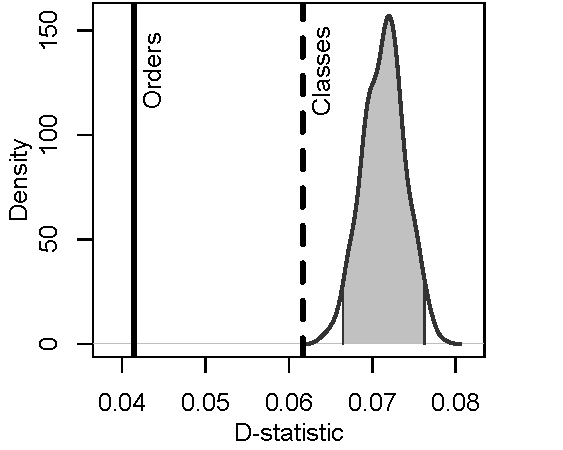
\includegraphics[scale=1]{figs/fig_dStat(3TP).pdf}
%DIFDELCMD <   \caption[Goodness of super-statistical theory fit]{%%%
\DIFdelendFL \DIFaddbeginFL 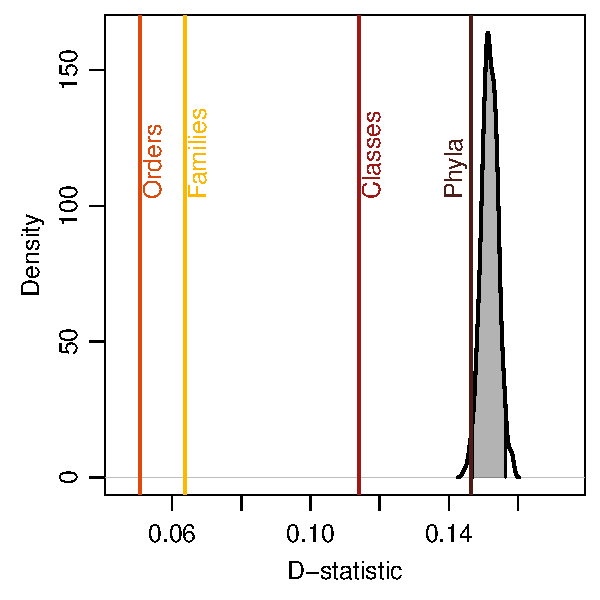
\includegraphics[scale=1]{../../fig_dStat.pdf}
  \caption[Goodness of superstatistical theory fit]{\DIFaddendFL Distribution of
    Kolmogorov-Smirnov (KS) statistics from randomly permuting genera
    within \DIFdelbeginFL \DIFdelFL{orders }\DIFdelendFL \DIFaddbeginFL \DIFaddFL{familes }\DIFaddendFL (gray shading represents 95\% confidence
    interval). Solid \DIFdelbeginFL \DIFdelFL{black line is }\DIFdelendFL \DIFaddbeginFL \DIFaddFL{colored lines are }\DIFaddendFL observed KS \DIFdelbeginFL \DIFdelFL{statistic }\DIFdelendFL \DIFaddbeginFL \DIFaddFL{statistics }\DIFaddendFL at
    \DIFdelbeginFL \DIFdelFL{the order
    level, while the dashed black line shows the observed KS statistic
    at the class level}\DIFdelendFL \DIFaddbeginFL \DIFaddFL{different taxonomic levels as indicated}\DIFaddendFL .}
  \label{fig:dStat}
\end{figure}

To further test the evolutionary coherence of \DIFdelbegin \DIFdel{orders }\DIFdelend \DIFaddbegin \DIFadd{families }\DIFaddend we conducted a
permutation experiment in which genera were randomly reassigned to
\DIFdelbegin \DIFdel{orders }\DIFdelend \DIFaddbegin \DIFadd{families }\DIFaddend while maintaining the number of genera in each \DIFdelbegin \DIFdel{order}\DIFdelend \DIFaddbegin \DIFadd{family}\DIFaddend . For
each permutation, we calculated the \DIFdelbegin \DIFdel{super-statistical prediction and
the
}\DIFdelend \DIFaddbegin \DIFadd{superstatistical prediction and
its }\DIFaddend Kolmogorov-Smirnov statistic. The permutation simulates a null
model in which common evolutionary history is stripped away (genera
are placed in random \DIFdelbegin \DIFdel{orders}\DIFdelend \DIFaddbegin \DIFadd{families}\DIFaddend ) but the total number of observed genera
per \DIFdelbegin \DIFdel{order }\DIFdelend \DIFaddbegin \DIFadd{family }\DIFaddend is held constant. \DIFdelbegin \DIFdel{Repeating this permutation }\DIFdelend \DIFaddbegin \DIFadd{Controlling for the total number of
genera per family is key because this could be purely an artifact of
an arbitrary taxonomic process \mbox{%DIFAUXCMD
\citep{yule1925, capocci2008} }%DIFAUXCMD
and genus
richness alone could be solely responsible for differences in the
$\beta_k$ across clades. Indeed, the number of genera in a family and
that family's $\beta_k$ value are correlated
(Fig. \ref{figSupp:betaByRich}). Thus we want to know if this
correlation alone accounts for all downstream superstatistical
results.
}

\DIFadd{Repeating the null permutation of genera in families }\DIFaddend 500 times yields
a null distribution of Kolmogorov-Smirnov statistics that is far
separated from the observed \DIFdelbegin \DIFdel{value }\DIFdelend \DIFaddbegin \DIFadd{values at the family and order levels
}\DIFaddend (Fig. \ref{fig:dStat}) suggesting \DIFaddbegin \DIFadd{that }\DIFaddend the good fit at \DIFdelbegin \DIFdel{the order level }\DIFdelend \DIFaddbegin \DIFadd{these levels }\DIFaddend is
not merely a statistical artifact of classification \DIFaddbegin \DIFadd{or the richness of
clades, }\DIFaddend but carries important biological information. \DIFaddbegin \DIFadd{Classes approach
the null and phyla are no different. It should also be noted that the
width of 95\% confidence interval of this null distribution is not far
from the distance between the Kolmogorov-Smirnov statistics of orders
versus families, suggesting that differences of fit between these
taxonomic levels is at least partially accounted for by the randomness
of the sampling distribution of Kolmogorov-Smirnov statistics.
}\DIFaddend 

\section{Discussion}

%% why orders
Our analysis makes no assumption that orders and families should
correspond to \DIFadd{superstatistical }\DIFaddend subsystems, but identifies them as the
appropriate level for marine invertebrates. Our study is the first to
demonstrate that complex patterns in the fluctuation of \DIFdelbegin \DIFdel{diversity resulting from the sequence of origination
and extinction events }\DIFdelend \DIFaddbegin \DIFadd{taxon richness
}\DIFaddend in the fossil record are the result of a simple underlying process
analogous to the statistical mechanisms by which complexity emerges in
large, non-equilibrium physical \citep{beck2004} and social systems
\citep{fuentes2009}.  We do so by identifying the biological scale at
which clades conform to locally independent dynamic equilibria in
fluctuations.  \DIFdelbegin \DIFdel{This scale is determined by the
process of niche conservatism \mbox{%DIFAUXCMD
\citep{roy2009range, hopkins2014} }%DIFAUXCMD
within
orders.  }\DIFdelend Equilibrium could result from many processes, including
neutrality \citep{macWilson, hubbell2001}, diversity-dependence
\DIFdelbegin \DIFdel{\mbox{%DIFAUXCMD
\citep{gavrilets2005, rabosky2009ecolLett} }%DIFAUXCMD
}\DIFdelend \DIFaddbegin \DIFadd{\mbox{%DIFAUXCMD
\citep{moen2014, foote2018} }%DIFAUXCMD
}\DIFaddend and processes that dampen---rather than
exacerbate---fluctuations in complex ecological networks
\citep{berlow2009}. \DIFaddbegin \DIFadd{These candidate processes are directly opposed to
the presumption of instability underlying the self-organized
criticality hypothesis for paleo biodiversity \mbox{%DIFAUXCMD
\citep{bak1993,
  sole1997}}%DIFAUXCMD
}\DIFaddend .

\DIFdelbegin \DIFdel{The distribution describing this process of evolution in }\DIFdelend \DIFaddbegin \DIFadd{We show that the distribution describing the evolution to different
}\DIFaddend equilibria between orders \DIFdelbegin \DIFdel{is clearly }\DIFdelend \DIFaddbegin \DIFadd{and families is }\DIFaddend Gamma (Fig. \ref{fig:pk_f}\DIFaddbegin \DIFadd{)}\DIFaddend .
A Gamma distribution, while consistent with multiple processes\DIFdelbegin \DIFdel{(e.g., \mbox{%DIFAUXCMD
\citep{cir1985}}%DIFAUXCMD
), }\DIFdelend \DIFaddbegin \DIFadd{, }\DIFaddend could
result from evolution of diversification rates across an adaptive
landscape that promotes niche conservatism and \DIFdelbegin \DIFdel{punctuated }\DIFdelend \DIFaddbegin \DIFadd{pulsed }\DIFaddend exploration of
niche space \DIFaddbegin \DIFadd{\mbox{%DIFAUXCMD
\citep{cir1985}}%DIFAUXCMD
}\DIFaddend .  Specifically, if $\beta_k$ values are
associated with a clade's \DIFdelbegin \DIFdel{physiological and life history
}\DIFdelend \DIFaddbegin \DIFadd{macroevolutionarily-relevant }\DIFaddend traits, and
those traits evolve via Ornstein-Uhlenbeck-like exploration of an
adaptive landscape, the resulting stationary distribution of $\beta_k$
will be Gamma \DIFdelbegin \DIFdel{\mbox{%DIFAUXCMD
\citep{cir1985, butler2004}}%DIFAUXCMD
}\DIFdelend \DIFaddbegin \DIFadd{\mbox{%DIFAUXCMD
\citep{cir1985}}%DIFAUXCMD
}\DIFaddend .  For macroevolutionary rates to vary
across an adaptive landscape, this landscape cannot be flat, and thus
niche conservatism \DIFdelbegin \DIFdel{punctuated }\DIFdelend \DIFaddbegin \DIFadd{around local optima in adaptive space interrupted
}\DIFaddend by adaptive exploration is \DIFdelbegin \DIFdel{inevitable \mbox{%DIFAUXCMD
\citep{newman1985adaptive}}%DIFAUXCMD
}\DIFdelend \DIFaddbegin \DIFadd{likely \mbox{%DIFAUXCMD
\citep{newman1985adaptive,
  gavrilets2004book}}%DIFAUXCMD
}\DIFaddend . The specifics of how this adaptive landscape is
shaped and is traversed by evolving clades \DIFdelbegin \DIFdel{will likely determine the specific distribution (e.g. Gamma versus Chi-squared, etc.) describing punctuated evolution
of clades' equilibria}\DIFdelend \DIFaddbegin \DIFadd{determine the exact form of
the distribution of $\beta_k$ volatilities, in the case of the marine
Phanerozoic resulting in a Gamma distribution}\DIFaddend . Our work thus motivates
\DIFaddbegin \DIFadd{further }\DIFaddend study of the trait spaces and evolutionary shifts consistent
with Gamma-distributed equilibria in \DIFdelbegin \DIFdel{diversity fluctuations}\DIFdelend \DIFaddbegin \DIFadd{richness fluctuation
volatilities}\DIFaddend .

%DIF < %% how this motivates future work in figuring out the details of
%DIF < %% biotic evolution that are important for driving stasis and
%DIF < %% punctuation
\DIFdelbegin \DIFdel{Our work highlights the importance of both }\DIFdelend \DIFaddbegin \DIFadd{We show that the pulsed shift to different equilibria between orders
and the families they subsume is sufficient to explain the
characteristically fat-tailed distribution of richness fluctuations
when the marine Phanerozoic invertebrate fauna is viewed as a whole
macrosystem.  Armed with an understanding of the statistical origin of
this diversification pattern we can explore which models of }\DIFaddend niche
conservatism and \DIFdelbegin \DIFdel{punctuated adaptive radiation in producing }\DIFdelend \DIFaddbegin \DIFadd{pulsed adaptive radiation are consistent with }\DIFaddend the
statistical behavior of the Phanerozoic\DIFdelbegin \DIFdel{; our theory
thus }\DIFdelend \DIFaddbegin \DIFadd{. Our statistical theory
}\DIFaddend provides new motivation for identifying the eco-evolutionary causes of
innovations between lineages and how those innovations are eventually
conserved within lineages. \DIFdelbegin \DIFdel{Armed with an understanding of the statistical behavior of
diversification we can }\DIFdelend \DIFaddbegin \DIFadd{Using the superstatistical prediction as a
theoretical baseline, we can also }\DIFaddend go on to \DIFdelbegin \DIFdel{examine mechanisms underlying
additional patterns in the mean trend of biodiversity through the
Phanerozoic. In particular, clades have been shown to }\DIFdelend \DIFaddbegin \DIFadd{identify and robustly
examine the mechanisms underlying deviations from statistical
theory. For example, some clades }\DIFaddend wax and wane systematically\DIFdelbegin \DIFdel{through time \mbox{%DIFAUXCMD
\citep{liow2007,
  quental2013}}%DIFAUXCMD
}\DIFdelend \DIFaddbegin \DIFadd{, and
possibly non-symmetrically, through time \mbox{%DIFAUXCMD
\citep{liow2007,
  foote2008paleobiol, quental2013}}%DIFAUXCMD
}\DIFaddend , a pattern that we cannot explain
with \DIFdelbegin \DIFdel{super-statistics
}\DIFdelend \DIFaddbegin \DIFadd{superstatistics }\DIFaddend alone.

%DIF < % note on how sstat could be applied to other questions in eco-evo.
Superstatistics could also be applied to other areas of evolution and
macroecology.  For example new phylogenetic models already consider
heterogeneous rates of diversification (e.g., \DIFdelbegin \DIFdel{\mbox{%DIFAUXCMD
\citep{rabosky2006laser}}%DIFAUXCMD
) }\DIFdelend \DIFaddbegin \DIFadd{\mbox{%DIFAUXCMD
\citep{rabosky2014}}%DIFAUXCMD
) as
expected between different subsystems}\DIFaddend . The superstatistics of clades
in adaptive landscapes could \DIFdelbegin \DIFdel{provide a means to build efficient }\DIFdelend \DIFaddbegin \DIFadd{motivate }\DIFaddend models that jointly predict
\DIFdelbegin \DIFdel{morphological change and diversification}\DIFdelend \DIFaddbegin \DIFadd{changes in traits and diversification, a research area currently
struggling with model inadequacy \mbox{%DIFAUXCMD
\citep{rabosky2017fisse}}%DIFAUXCMD
}\DIFaddend . This
framework could also provide a new paradigm in modeling the
distributions of \DIFdelbegin \DIFdel{diversity, abundance}\DIFdelend \DIFaddbegin \DIFadd{richness, abundance, }\DIFaddend and resource use in non-neutral
communities \DIFaddbegin \DIFadd{which can be viewed as emerging from the combination of
locally equilibrium subsystems}\DIFaddend . Non-neutral models in ecology are
criticized for their over-parameterization \citep{rosindell2011}, yet
a persistent counter argument to neutral theory \citep{hubbell2001} is
the unrealistic assumption of ecological equivalency \DIFdelbegin \DIFdel{\mbox{%DIFAUXCMD
\citep{chave2004neutral} }%DIFAUXCMD
}\DIFdelend and poor
prediction of real dynamics \DIFdelbegin \DIFdel{\mbox{%DIFAUXCMD
\citep{ricklefs2006neutral}}%DIFAUXCMD
}\DIFdelend \DIFaddbegin \DIFadd{\mbox{%DIFAUXCMD
\citep{rosindell2011}}%DIFAUXCMD
}\DIFaddend . If ecosystems are
viewed as the \DIFdelbegin \DIFdel{super-position }\DIFdelend \DIFaddbegin \DIFadd{superposition }\DIFaddend of many individualistically evolving
clades, each exploiting the environment differently and thus obeying a
different set of \DIFdelbegin \DIFdel{non-equivalent }\DIFdelend statistics, then diversity dynamics could be
parsimoniously predicted with superstatistics while incorporating real
biological information on ecological differences between taxa.

Superstatistics is a powerful tool to derive macro-scale predictions
from locally fluctuating sub-systems whose evolution is driven by
interesting, but complex and difficult to model, biological
mechanisms. As such, applications of superstatistics \DIFdelbegin \DIFdel{from islands to populations to clades }\DIFdelend \DIFaddbegin \DIFadd{to a wide variety
of patterns in ecological and evolutionary systems }\DIFaddend are ripe for
exploration.

\section{Methods and Materials}

\DIFaddbegin \DIFadd{All data processing and analyses were preformed in R \mbox{%DIFAUXCMD
\citep{rcite} }%DIFAUXCMD
and all code needed to reproduce our study are provided, with added
explanation, in supplemental Appendix A.}

\subsection{Paleobiology Database data download and filtering}

\DIFadd{Data on individual fossil occurrences and the ecospace characteristics
of Phanerozoic marine invertebrates }\DIFaddend were downloaded from the
Paleobiology Database (PBDB; \DIFdelbegin \DIFdel{www.pbdb.org) on 28 May 2013. }\DIFdelend \DIFaddbegin \newline\texttt{\DIFadd{https://paleobiodb.org}}\DIFadd{) on 16
November 2018 via the database's API (data retrieval and processing
script available in the supplement). }\DIFaddend Collections were filtered using
the same approach as Alroy \citep{alroy08} to insure that only well
preserved marine invertebrate occurrences were used in subsequent
\DIFdelbegin \DIFdel{analysis
resulting in 221202 genus }\DIFdelend \DIFaddbegin \DIFadd{analyses. This filtering resulted in 815,222 unique genus-level
}\DIFaddend occurrences. These were further filtered to exclude those occurrences
without \DIFdelbegin \DIFdel{order-level }\DIFdelend \DIFaddbegin \DIFadd{family-level }\DIFaddend taxonomy and those collections with age estimate
resolutions outside the \DIFdelbegin \DIFdel{10my default
bins of the PBDB resulting in 189516 occurrencesleft for analysis. To
avoid basic sampling concerns we excluded the }\DIFdelend \DIFaddbegin \DIFadd{11MY time bins proposed by Alroy
\mbox{%DIFAUXCMD
\citep{alroy08} }%DIFAUXCMD
resulting in 454,033 occurrences. Time bins were
compiled from }{\tt \DIFadd{http://fossilworks.org}} \DIFadd{with a custom script
reproduced in the supplement. The first and last of these time bins,
corresponding to the }\DIFaddend earliest Cambrian and the latest Cenozoic\DIFdelbegin \DIFdel{.
}\DIFdelend \DIFaddbegin \DIFadd{, were
excluded from analysis because their sampling completeness (see below)
could not be assessed.
}\DIFaddend 


\DIFaddbegin \subsection{\DIFadd{Correcting for imperfect and potentially biased sampling}}
\DIFaddend \label{sec:3TP}
We use a new and flexible method \DIFdelbegin \DIFdel{, described below, }\DIFdelend to correct for known sampling
\DIFaddbegin \DIFadd{incompleteness and }\DIFaddend biases in publication-based specimen databases
\citep{alroy08, alroy2010}. \DIFdelbegin \DIFdel{We were motivated to use this method
because rarefaction has been shown to under-perform compared to the more data-intensive shareholder quorum subsampling (SQS) method
\mbox{%DIFAUXCMD
\citep{alroy2010}}%DIFAUXCMD
.  However, subsampling cannot be applied to small
orders (i.e. the majority) because SQS becomes increasingly unreliable
as sample size decreases \mbox{%DIFAUXCMD
\citep{alroy2010} }%DIFAUXCMD
}\DIFdelend \DIFaddbegin \DIFadd{Incompleteness is inherent in all
biodiversity samples, the fossil record being no exception
\mbox{%DIFAUXCMD
\citep{miller1996, foote2016, starrfelt2016, close2018}}%DIFAUXCMD
.  In addition
to incompleteness, bias may result from preferential publication of
novel taxa \mbox{%DIFAUXCMD
\citep{alroy2010} }%DIFAUXCMD
which exacerbates the difference between
poorly-sampled and well-sampled time periods}\DIFaddend . We therefore develop a
simple \DIFdelbegin \DIFdel{method based on first correcting for detection bias }\DIFdelend \DIFaddbegin \DIFadd{two-step method: we first correct genus richness for incomplete
sampling }\DIFaddend using the ``\DIFdelbegin \DIFdel{three timer}\DIFdelend \DIFaddbegin \DIFadd{three-timer}\DIFaddend '' correction \citep{alroy08} \DIFdelbegin \DIFdel{in which the rate }\DIFdelend \DIFaddbegin \DIFadd{and then
further correct this three-timer richness estimate by accounting for
any correlation between the number of genera and the number of
publications in a time period.
}

\DIFadd{The three-timer correction estimates the probability }\DIFaddend of failure to
observe a genus \DIFdelbegin \DIFdel{is estimated }\DIFdelend \DIFaddbegin \DIFadd{in a given time period $p_t$ as the number of times
any genus is recorded before and after that period but not during,
divided }\DIFaddend by the number of \DIFdelbegin \DIFdel{times a gap occurs in the occurrence history of each genus. }\DIFdelend \DIFaddbegin \DIFadd{genera whose occurrence histories span the
period $t$.  To calculate the sampling-corrected richness
$\hat{D}_{kt}$ of a clade $k$ in the time period in question, the
observed genera within that clade and time period are divided by
$1 - p_t$ and their occurrences summed:
}\begin{equation}
  \DIFadd{\hat{D}_{kt} = \sum_{j \in k} \frac{I_{jt}}{1 - p_t}
}\end{equation}
\DIFadd{where $j \in k$ designates genera in clade $k$ and $I_{jt}$ is an
indicator equal to 1 if genus $j$ occurs in time period $t$.
}

\DIFadd{$\hat{D}_{kt}$ is the maximum likelihood estimator of richness in a
simple occupancy through time type model assuming binomial sampling
\mbox{%DIFAUXCMD
\citep{royleDorazio}}%DIFAUXCMD
, and in that way mimics other proposed methods
for the fossil record \mbox{%DIFAUXCMD
\citep{foote2016, starrfelt2016}}%DIFAUXCMD
. We avoid
parametrically modeling the sampling process through time by instead
taking a sliding window of time bins from the Cambrian to the
Cenozoic. It should be noted that the three-timer correction compares
favorably to other similar methods to account for imperfect detection
\mbox{%DIFAUXCMD
\citep{alroy2014}
}%DIFAUXCMD
}

\DIFaddend To eliminate further bias due to preferential publication of novel
taxa \DIFdelbegin \DIFdel{we divide observed }\DIFdelend \DIFaddbegin \DIFadd{\mbox{%DIFAUXCMD
\citep{alroy2010} }%DIFAUXCMD
we divide the three-timer-corrected }\DIFaddend number of
genera per \DIFdelbegin \DIFdel{order }\DIFdelend \DIFaddbegin \DIFadd{family }\DIFaddend per time period by the expected number of genera
given publications in that time period.  The expected number is
calculated by regressing the log-transformed \DIFaddbegin \DIFadd{three-timer-corrected
}\DIFaddend number of genera on log-transformed number of publications. There is
\DIFaddbegin \DIFadd{only }\DIFaddend a weak trend toward higher \DIFdelbegin \DIFdel{diversity }\DIFdelend \DIFaddbegin \DIFadd{richness }\DIFaddend with more publications
(Fig. \DIFdelbegin \DIFdel{\ref{fig:divByPub}}\DIFdelend \DIFaddbegin \DIFadd{\ref{figSupp:divByPub}}\DIFaddend ) meaning that the most important correction
comes from the three timer correction.

Our new method \DIFdelbegin \DIFdel{effectively }\DIFdelend re-scales each genus occurrence from 0 \DIFdelbegin \DIFdel{/}\DIFdelend \DIFaddbegin \DIFadd{or }\DIFaddend 1 (absent \DIFdelbegin \DIFdel{/present) , }\DIFdelend \DIFaddbegin \DIFadd{or
present) }\DIFaddend to a weighted number continuously ranging between 0 and
1. \DIFdelbegin \DIFdel{This }\DIFdelend \DIFaddbegin \DIFadd{Because these weighted numbers represent sampling and
bias-corrected }{\it \DIFadd{occurrences}} \DIFadd{we can add them arbitrarily,
corresponding to the membership of any given genus in any given higher
taxonomic group.  We must, however, choose a taxonomic level at which
to evaluate the relationship between richness and publications; we
choose the level of family because this is the most finely resolved
option.
}

\DIFadd{We opt not to use subsampling methods \mbox{%DIFAUXCMD
\citep{miller1996, alroy2010,
  kocsis2018} }%DIFAUXCMD
because these approaches would not be advisable for
clades with few genera. However, our new }\DIFaddend method achieves similar
results to \DIFdelbegin \DIFdel{more computationally
intensive sub-sampling procedures \mbox{%DIFAUXCMD
\citep{alroy08, alroy2010}}%DIFAUXCMD
}\DIFdelend \DIFaddbegin \DIFadd{subsampling procedures at the global scale across all
clades}\DIFaddend . We directly compare our predicted time series of global
\DIFdelbegin \DIFdel{genus diversity
}\DIFdelend \DIFaddbegin \DIFadd{fluctuations in genus richness }\DIFaddend with results derived from \DIFdelbegin \DIFdel{SQS \mbox{%DIFAUXCMD
\citep{alroy2010} }%DIFAUXCMD
and the raw data
(Fig. \ref{fig:supp_3TPub}) }\DIFdelend \DIFaddbegin \DIFadd{rarefaction
and shareholder quorum subsampling (SQS) in Figure
\ref{figSupp:3TPub}}\DIFaddend .  Our method shows \DIFaddbegin \DIFadd{very }\DIFaddend minor differences with
\DIFdelbegin \DIFdel{the SQS prediction, However, these }\DIFdelend \DIFaddbegin \DIFadd{these subsampling-based predictions and any }\DIFaddend discrepancies do not
impact the \DIFaddbegin \DIFadd{statistical }\DIFaddend distribution of fluctuations
(Fig. \DIFdelbegin \DIFdel{\ref{fig:supp_3TPub})and
super-statistical analysis on uncorrected PBDB data (see section
\ref{sec:rawPBDB}) produces a similar result to the analysis on
corrected PBDB data presented in the main text}\DIFdelend \DIFaddbegin \DIFadd{\ref{figSupp:3TPub})}\DIFaddend.

\DIFaddbegin \subsection{\DIFadd{Superstatistical methods}} \DIFaddend \label{sec:numMeth}
\DIFaddbegin 

\DIFaddend We first derive the \DIFdelbegin \DIFdel{super-statistical }\DIFdelend \DIFaddbegin \DIFadd{superstatistical }\DIFaddend distribution $P(x)$ by fitting
Gaussian distributions to clade-level distributions of fluctuations
$p_k(x)$, extracting the \DIFdelbegin \DIFdel{variances }\DIFdelend inverse variances $\beta_k$ of those
$p_k(x)$, testing the best function to describe the distribution of
$\beta_k$, and then integrating
$P(x) = \int_{\beta}p_k(x | \beta) f(\beta)$. This process allows \DIFdelbegin \DIFdel{to
}\DIFdelend \DIFaddbegin \DIFadd{no
}\DIFaddend free parameters to hone the fit of $P(x)$ to the data.  However, each
inverse variance must of course be estimated for each clade\DIFaddbegin \DIFadd{, making
its good fit to data all the more surprising}\DIFaddend .  To do so we use least
squares instead of maximum likelihood because the asymmetric
fluctuation distributions of small clades were more reliably fit with
curve fitting than with \DIFdelbegin \DIFdel{the maximum likelihoodestimator}\DIFdelend \DIFaddbegin \DIFadd{maximum likelihood}\DIFaddend .

We \DIFdelbegin \DIFdel{then }\DIFdelend \DIFaddbegin \DIFadd{also }\DIFaddend estimated $P(x)$ directly from the \DIFdelbegin \DIFdel{raw }\DIFdelend \DIFaddbegin \DIFadd{family-level }\DIFaddend data using
maximum likelihood to compare the fit of our \DIFdelbegin \DIFdel{super-statistical }\DIFdelend \DIFaddbegin \DIFadd{superstatistical
}\DIFaddend prediction and that of a simple Gaussian distribution using AIC. To
calculate a likelihood-based confidence interval on our prediction we
bootstrapped the data, subsampling fluctuations with replacement from
all \DIFdelbegin \DIFdel{orders
combined, and calculating AIC of the
superstatistical and Gaussian
models on these bootstrapped datasets}\DIFdelend \DIFaddbegin \DIFadd{families and fit superstatistics using maximum likelihood to the
aggregated fluctuation distribution of each bootstrap replicate}\DIFaddend .

\bibliographystyle{Science}
\DIFdelbegin %DIFDELCMD < \bibliography{../superStat}
%DIFDELCMD < %%%
\DIFdelend \DIFaddbegin \bibliography{../../superStat}
\DIFaddend 


\section*{Acknowledgments}
\begin{itemize}
\item[{\bf General:}] We thank John Harte, Rosemary Gillespie, Linden
  Schneider, \DIFdelbegin \DIFdel{and }\DIFdelend Jun Ying Lim\DIFaddbegin \DIFadd{, and David Jablonski }\DIFaddend for helpful
  discussion. We thank \DIFdelbegin \DIFdel{the
  }\DIFdelend \DIFaddbegin \DIFadd{Aaron Clauset and four anonymous reviewers for
  greatly improving the quality of this manuscript. We thank the }\DIFaddend many
  contributors to the Paleobiology Database for making data
  available. \DIFaddbegin \DIFadd{The current work derives from the PhD dissertation of
  AJR \citep{romingerPhD}.} \DIFaddend
\item[{\bf Funding:}] AJR thanks funding from Fulbright Chile, the
  National Science Foundation Graduate Research Fellowship Program and
  the Omidyar Program at the Santa Fe Institute; MAF thanks FONDECYT
  1140278; PM thanks CONICYT PFB-023, ICM-P05-002 and FONDECYT
  1161023.
\item[{\bf Author contributions:}] AJR, MAF and PAM designed the
  study; AJR and MAF preformed the analyses; AJR, MAF and PAM
  interpreted the results and wrote the manuscript.
\item[{\bf Competing interests:}] none.
\item[{\bf Data and materials availability:}] Data are available
  through \DIFaddbegin \DIFadd{the Paleobiology Database (}\DIFaddend
  {\tt paleobiodb.org}\DIFdelbegin \DIFdel{, analysis scripts
  }\DIFdelend \DIFaddbegin \DIFadd{) and all code needed to interface
    with the }{\tt \DIFadd{paleobiodb.org}} \DIFadd{API, process,
    clean, and ultimately analyze the data }\DIFaddend are available
  online at \\
  {\tt github.com/ajrominger/paleo\_supStat}. \DIFaddbegin
  \DIFadd{This github repository also hosts the exact download from
  }{\tt \DIFadd{paleobiodb.org}} \DIFadd{used in this analysis. All
    required scripts are also available and explained in supplemental
    Appendix A.  }\DIFaddend \end{itemize}


\clearpage
\setcounter{page}{1}
\nolinenumbers

\newcommand{\beginsupplement}{%
  \setcounter{table}{0}
  \renewcommand{\thetable}{S\arabic{table}}%
  \setcounter{figure}{0}
  \renewcommand{\thefigure}{S\arabic{figure}}%
  \setcounter{section}{0}
  \renewcommand{\thesection}{S\arabic{section}}%
}

\beginsupplement

\begin{center}
{\LARGE \bf Supplementary materials}
\end{center}
\vspace{2em}

\section{Limit distribution of a time-averaged homogeneous
  origination-extinction process}
\label{sec:suppLimitDist}
\DIFaddbegin 

\DIFaddend Fossil taxa gain and lose \DIFdelbegin \DIFdel{taxa }\DIFdelend \DIFaddbegin \DIFadd{genera }\DIFaddend according to an
origination-extinction process. We assume that most fossil occurrences
of a taxon come from the period of its history when it is dominant and
in steady state. In a time slice of duration $\tau$ during such a
period of steady state the latent per capita rates of origination and
extinction would be equal (i.e. $\lambda = \mu \equiv \rho$) and the
number of origination or extinctions events (call such events $Y$)
each follow an inhomogeneous Poisson process with rate $\rho N_t$
where $N_t$ is the number of \DIFdelbegin \DIFdel{species or }\DIFdelend genera in the taxon of interest at time
$t$. Allowing $N_t$ to vary smoothly with time, and \DIFdelbegin \DIFdel{invoking the communicative property of the Poisson distribution}\DIFdelend \DIFaddbegin \DIFadd{recognizing that
the sum of Poisson random variables remains Poisson}\DIFaddend , we arrive at the
number $Y$ of extinction \emph{or} origination events in $\tau$ being
distributed
\begin{equation}
  \label{eq:eventPois1}
  Y \sim \text{Pois}\left(\rho \int_{t=0}^\tau N(t) dt\right).
\end{equation}
Under the steady state assumption we can approximate $N(t)$ by
$\bar{N}$, the steady state \DIFdelbegin \DIFdel{diversity}\DIFdelend \DIFaddbegin \DIFadd{richness}\DIFaddend , leading to
\begin{equation}
  \label{eq:eventPois2}
  Y \sim \text{Pois}(\rho \bar{N} \tau).
\end{equation}

\DIFdelbegin \DIFdel{Assuming the $\tau$ of each time period in the Paleobiology Database
or Sepkoski's compendium to be approximately equal (i. e. equal
durations of major asymptotic units) then the }\DIFdelend \DIFaddbegin \DIFadd{This Poisson distribution is asymptotically Gaussian, which is a more
appropriate distribution for our sampling and bias-corrected richness
estimates because these estimates are not integer-valued but rather
continuous random variables. Furthermore, because we use standard time
periods of average duration $\tau = 11\text{MY}$ the the }\DIFaddend distribution
of fluctuations within taxa will be \DIFaddbegin \DIFadd{independent of the specific time
periods considered. }\DIFaddend The Gaussian asymptotics of time-averaged
birth-death processes have been proven and explored elsewhere as well
\DIFdelbegin \DIFdel{\mbox{%DIFAUXCMD
\citep{keilson1970,
  grassmann1987}}%DIFAUXCMD
}\DIFdelend \DIFaddbegin \DIFadd{\mbox{%DIFAUXCMD
\citep{grassmann1987}}%DIFAUXCMD
}\DIFaddend .


\section{\DIFadd{Evaluation of sampling bias correction methods}}
\label{sec:suppBiasEval}

\DIFaddbegin \DIFadd{Our sampling and bias-correction method first accounts for imperfect
detection within a binomial sampling framework as described in the
main text, and then further corrects for potential publication bias
using simple log-log regression.  We reproduce that regression of
log-richness versus log-number of publications here
(Fig. \ref{figSupp:divByPub}). }\DIFaddend 

\DIFaddbegin \begin{figure}[!hp]
  \centering
  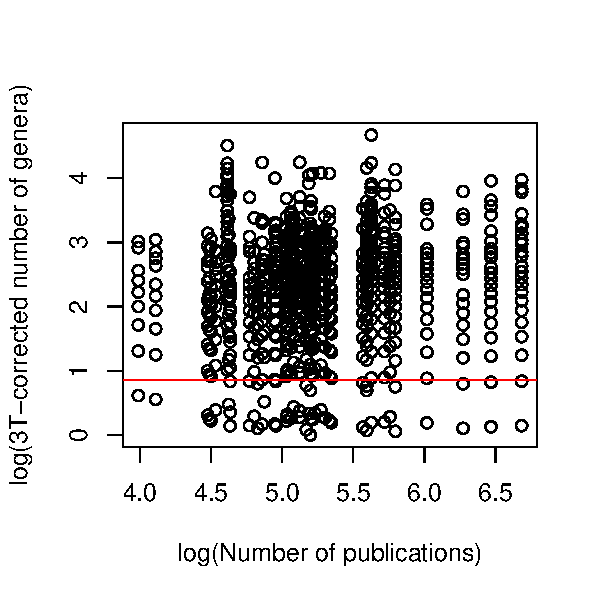
\includegraphics[width=0.4\textwidth]{../../figSupp_divByPub.pdf}
  \caption{\DIFaddFL{Relationship between number of publications and genus
    richness at the family level as recorded by the PBDB.}}
  \label{figSupp:divByPub}
\end{figure}


\DIFadd{We compare our sampling and bias-correction method to other more
established approaches. Specifically we use the newly available R
package }{\it \DIFadd{divDyn}} \DIFadd{\mbox{%DIFAUXCMD
\citep{kocsis2018} }%DIFAUXCMD
to produce subsampling-based
richness estimates for the Phanerozoic timeseries of marine
invertebrates. In Figure \ref{figSupp:3TPub} we compare classical
rarefaction and shareholder quorum subsampling (SQS) with our
method. All samples were rarified to 120 occurrences, which is
approximately the maximum possible rarefied sample size across all
time bins, and the SQS quorum was set to 0.75 to similarly approximate
this common sampling denominator across time bins. For both
rarefaction and SQS we averaged 50 subsampled replicates.}\DIFaddend 


\DIFaddbegin \begin{figure}[!hp]
  \centering
  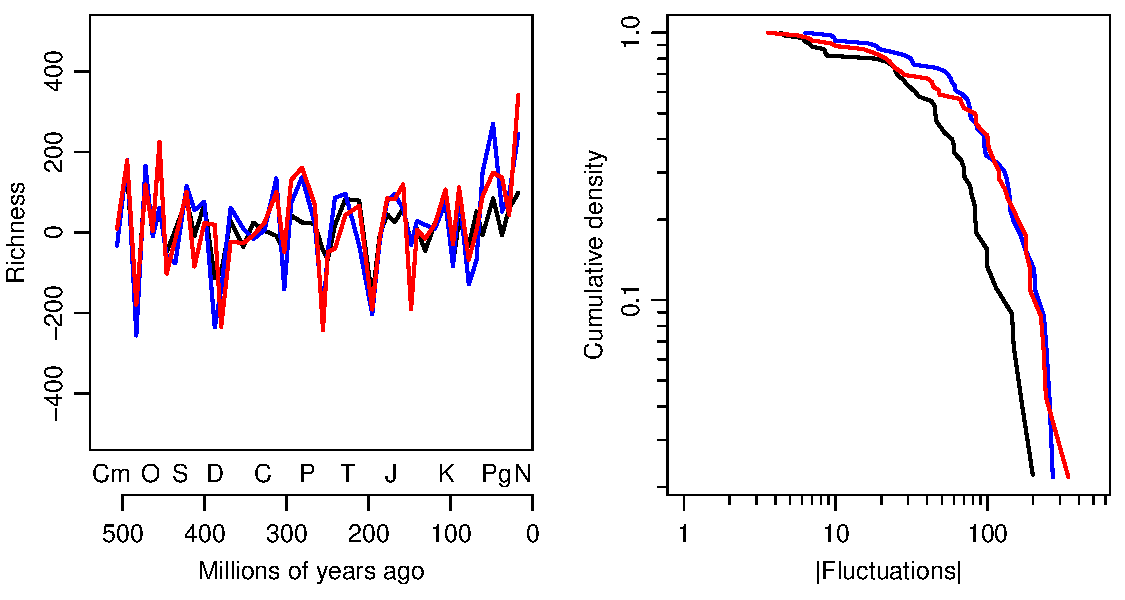
\includegraphics[width=0.7\textwidth]{../../figSupp_divEstComp.pdf}
  \caption{\DIFaddFL{Comparison of rarefaction (black line) and SQS (blue)
    with our three-timer and publication bias correction method
    (red). The time-series of all marine invertebrate genera shows
    general agreement with the only major deviations toward the modern
    (A). Despite these differences the distribution of fluctuations in
    genus richness across all marine invertebrates show good agreement
    (B).}}
  \label{figSupp:3TPub}
\end{figure}


\section{\DIFadd{Understanding deviations from superstatistics at higher
  taxonomic levels}}
\label{sec:suppSstatTaxLevels}

\DIFadd{To explore why deviations from super statistics increase with
increasing taxonomic level we explore how the distributions of
richness fluctuations $p_k(x | \beta_k)$ and fluctuation volatilities
$f(\beta_k)$ change with changing taxonomic level. We find that
richness fluctuation distributions experience increasing frequencies
of outliers (increasing kurtosis) with higher taxonomic level
(Fig. \ref{figSupp:pkx_allTaxa}). We also find that observed
fluctuation volatility distributions increasingly depart from a Gamma
distribution at the levels of classes and phyla
(Fig. \ref{figSupp:fbeta_allTaxa}).}\DIFaddend 


\DIFaddbegin \begin{figure}[!hp]
  \centering
  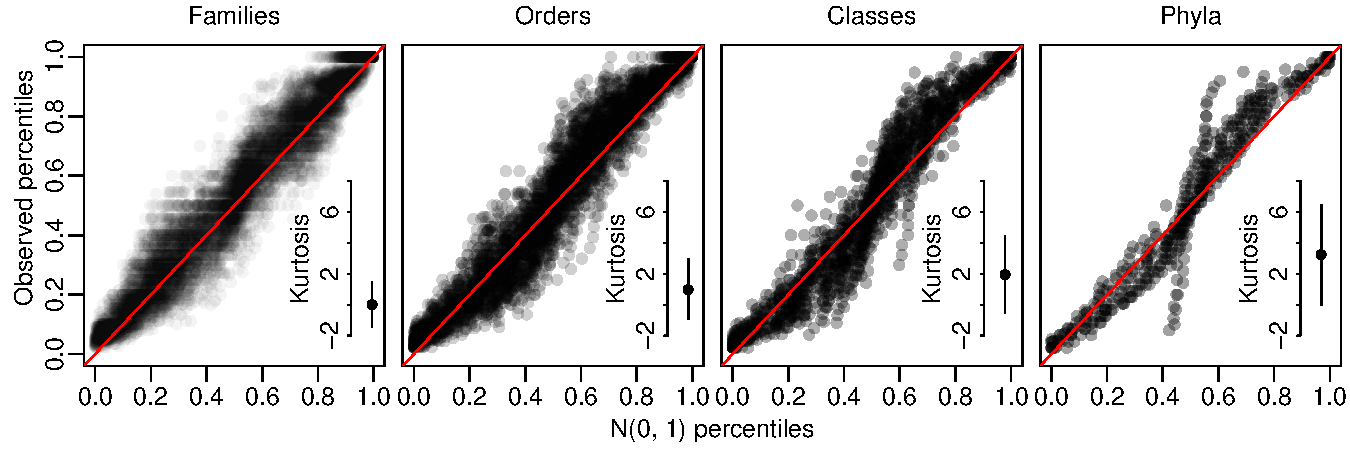
\includegraphics[width=0.8\textwidth]{../../figSupp_pkx_allTaxa.pdf}
  \caption{\DIFaddFL{Change in within clade richness fluctuation distributions
    with increasing taxonomic level. The percentile-percentile plots
    show how the percentiles of observed re-scaled fluctuation
    distributions compare to expected percentiles from a Gaussian
    distribution with mean 0 and variance 1. We can see that families
    conform to a linear relationship while higher taxa, even at the
    order level, begin to show s-shaped relationships. Inset plots
    show how kurtosis increases from 0 (the value for a Gaussian
    distribution) at the family level to increasingly larger values
    at higher taxonomic levels.}}
  \label{figSupp:pkx_allTaxa}
\end{figure}

\DIFaddbegin \begin{figure}[!hp]
  \centering
  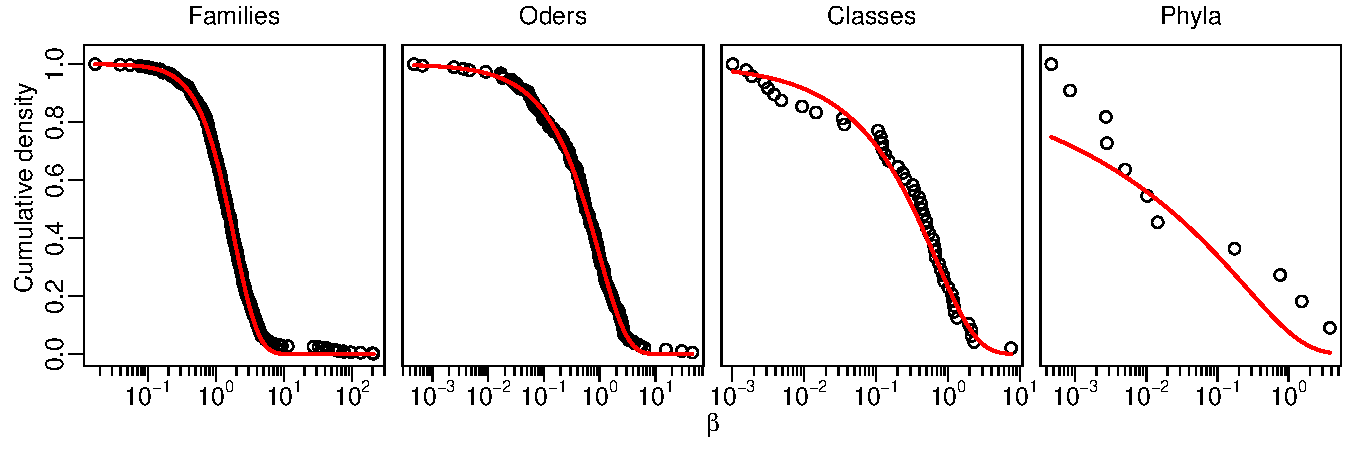
\includegraphics[width=0.8\textwidth]{../../figSupp_fbeta_allTaxa.pdf}
  \caption{\DIFaddFL{Change in the distributions of $\beta_k$ across clades of
    increasing taxonomic level. Points are observed $\beta_k$ values
    and red lines are the best-fit Gamma distributions. Deviations
    increase particularly at the class and phylum levels.}}
  \label{figSupp:fbeta_allTaxa}
\end{figure}




\DIFaddbegin \section{\DIFadd{Ecospace occupation of higher taxa}}
\label{sec:suppGuilds} 

\DIFadd{We posit that part of the increasing divergence between
superstatistics and observed fluctuations and the increase in
fluctuation outliers at higher taxonomic levels is that these higher
taxa increasingly aggregate disparate types of organisms. One way to
evaluate this idea is to count the ecospace hypercubes
\mbox{%DIFAUXCMD
\citep{bambach1983, bambach2007, bush2007} }%DIFAUXCMD
occupied by taxa at
different levels. We use the ecological characteristics reported by
the PBDB: taxon environment, motility, life habit, vision, diet,
reproduction, and ontogeny. In Figure \ref{figSupp:eeSpaceOcc} we find
that families comprise, on average, 1 hypercube, families comprise 2
hypercubes on average, and classes and phyla comprise many more.}


\DIFaddbegin \begin{figure}[!hp]
  \centering
  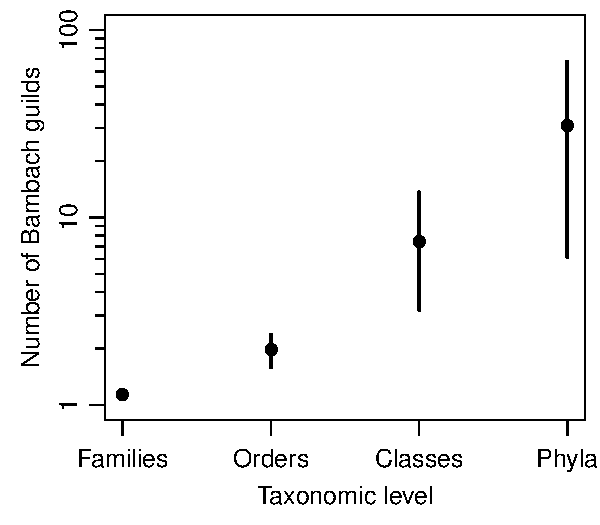
\includegraphics[width=0.4\textwidth]{../../figSupp_eeSpaceOcc.pdf} 
  \caption{\DIFaddFL{Relationship between number of ecospace hypercubes occupied
    and taxonomic level.}}
  \label{figSupp:eeSpaceOcc}
\end{figure}


\section{\DIFadd{Relationship between $\beta_k$ and clade richness}}
\label{sec:suppBetaRichness} 

\DIFadd{There is likely to be a relationship between richness of clade $k$ and
its fluctuation volatility $\beta_k$ because both extinction and
origination (i.e. the formation of new genera) contribute to
volatility. Thus we expect that higher variance in richness
fluctuations (i.e. smaller $\beta_k = 1/\text{variance}$) will be
correlated with higher richness.  Indeed, Figure
\ref{figSupp:betaByRich} shows this to be true. In the main text we
use permutation to evaluate whether this correlation is responsible
for the observed good fit of superstatistics, and find that this
correlation alone is not sufficient.
}

\DIFaddbegin \begin{figure}[!hp]
  \centering
  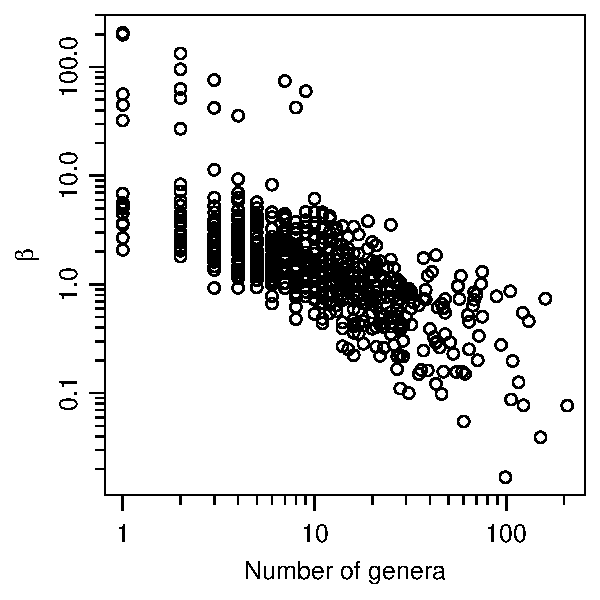
\includegraphics[width=0.4\textwidth]{../../figSupp_betaByRich.pdf} 
  \caption{\DIFaddFL{Relationship between fluctuation volatility $\beta_k$ and
    genus richness at the family level.}}
  \label{figSupp:betaByRich}
\end{figure}


\clearpage 

\setlength{\voffset}{0cm}
\setlength{\hoffset}{0cm}
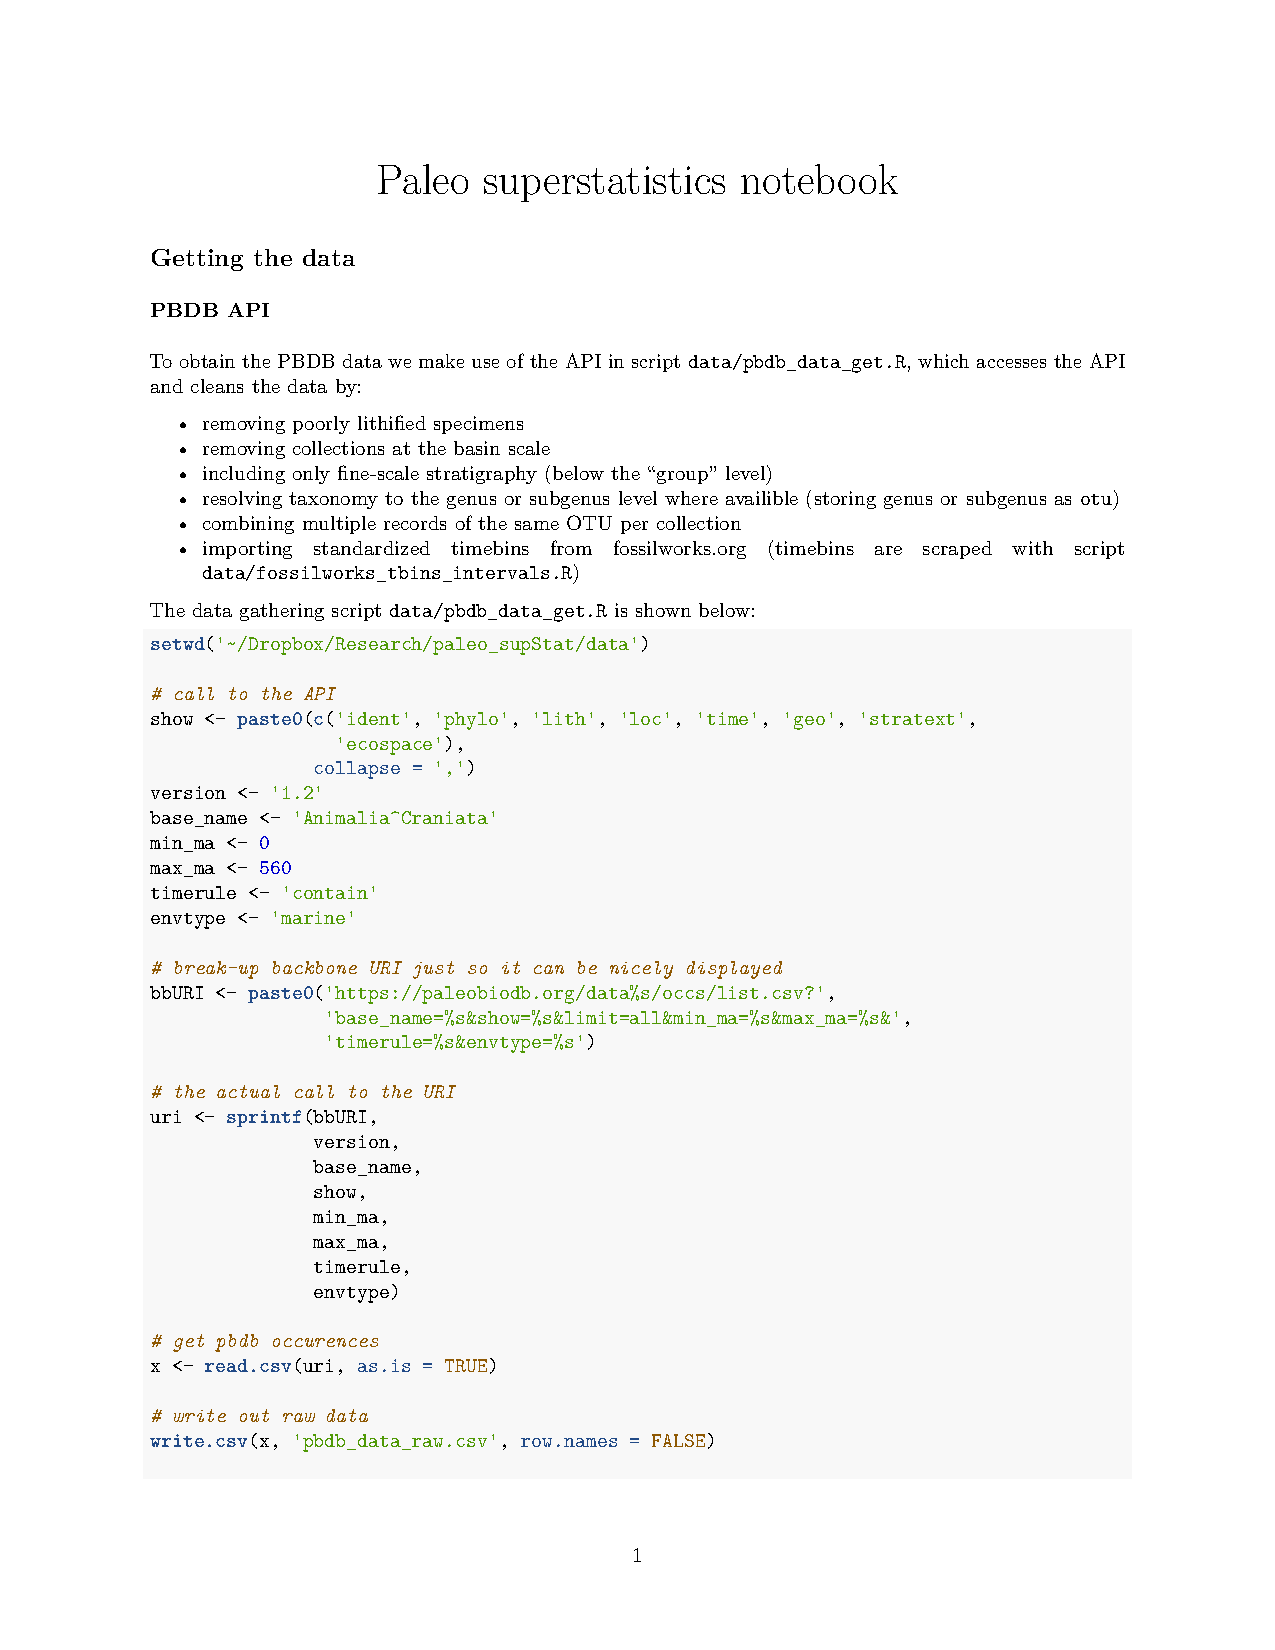
\includepdf[pages=-]{../../../sstat_notebook.pdf}

% \input{../../../sstat_notebook_include.tex}
\end{document}

